\documentclass[12pt,a4paper]{article}
\usepackage[utf8]{inputenc}
\usepackage{graphicx}
\usepackage{amsmath}
\usepackage{amsthm}
\usepackage{amssymb}
\usepackage{hyperref}
\usepackage{subfig}
\usepackage{multirow}

\begin{document}

\begin{titlepage}
	\centering
	
\includegraphics[width=0.15\textwidth]{IIIT-B_logo.jpg}\par\vspace{1cm}
	{\scshape\LARGE International Institute of Information Technology Bangalore \par}
	\vspace{1cm}
	{\scshape\Large Project Progress Report\par}
	{\Large DS/NC/ESD 863 Machine Perception\par}
	\vspace{1.5cm}
	{\huge\bfseries Vehicle Driving Assistant \par}
	\vspace{2cm}	   
	{\Large\itshape Akanksha Dwivedi - MT2016006\par}
	{\Large\itshape Anoop Toffy - MT2016016\par}
	{\Large\itshape Athul Suresh - MT2016030\par}
	{\Large\itshape Tarini Chandrashekhar - MT2016144\par}
	\vfill
	{\huge Group 7 \par}
	\vfill
	Guide : \par
	Prof. Dinesh Babu Jayagopi 

	\vfill

% Bottom of the page
	{\large \today\par}
\end{titlepage}


\tableofcontents
%\listoffigures
%\listoftables
\newpage


\begin{enumerate}
  \item Morphological transformations are some simple operations based on the image shape. It is normally performed on binary images. It needs two inputs, one is the original image, second one is called structuring element or kernel which decides the nature of operation. Two basic morphological operators are Erosion and Dilation. Then its variant forms like Opening, Closing, Gradient etc also comes into play.
    \begin{center}
        \includegraphics{j}
    \end{center}
    \begin{enumerate}
    \item \textbf{Erosion}
    The basic idea of erosion is to erode away the boundaries of foreground object. The kernel slides through the image (as in 2D convolution). A pixel in the original image (either 1 or 0) will be considered 1 only if all the pixels under the kernel is 1, otherwise it is eroded (made to zero).

    So, all the pixels near boundary will be discarded depending upon the size of kernel. The thickness or size of the foreground object decreases or simply white region decreases in the image. It is useful for removing small white noises, detach two connected objects etc.
    \begin{center}
        \includegraphics{erosion}
    \end{center}
    \item \textbf{Dilation}
    It is just opposite of erosion. Here, a pixel element is '1' if atleast one pixel under the kernel is '1'. So, it increases the white region in the image or size of foreground object increases. Normally, in cases like noise removal, erosion is followed by dilation. Because, erosion removes white noises, but it also shrinks our object. So, we dilate it. Since noise is gone, they won't come back, but our object area increases. It is also useful in joining broken parts of an object. 
    \begin{center}
        \includegraphics{dilation}
    \end{center}
    \item \textbf{Opening}
    Opening is just another name of erosion followed by dilation. It is useful in removing noise.
    \begin{center}
        \includegraphics{opening}
    \end{center}
    \item \textbf{Closing}
    Closing is reverse of Opening, Dilation followed by Erosion. It is useful in closing small holes inside the foreground objects, or small black points on the object. \begin{center}
        \includegraphics{closing}
    \end{center}
    \item \textbf{Morphological Gradient}
    It is the difference between dilation and erosion of an image.
    \begin{center}
        \includegraphics{gradient}
    \end{center}
    \end{enumerate}
    \pagebreak
\end{enumerate}

\begin{enumerate}
  \item Pre-processing Techniques:
    \begin{enumerate}
    \item \textbf{Method 1:Blob Detection Using LOG, DOG, DOH}
    \begin{enumerate}
        \item In the Blob Detection Technique, the Laplacian Of Gaussian(LOG), Difference Of Gaussian(DOG) and the Determinant of Hessian(DOH) was found out with arguments \textbf{max\_sigma} as 30, \textbf{num\_sigma} as 10 and \textbf{threshold} as .1 in the input frames. It was observed that the LOG and DOG was detecting the potholes, additional to the noise in the frames and the DOH methodology detected only a fraction of the potholes.
    \end{enumerate}
    
    \begin{figure}[ht!]
        \centering
        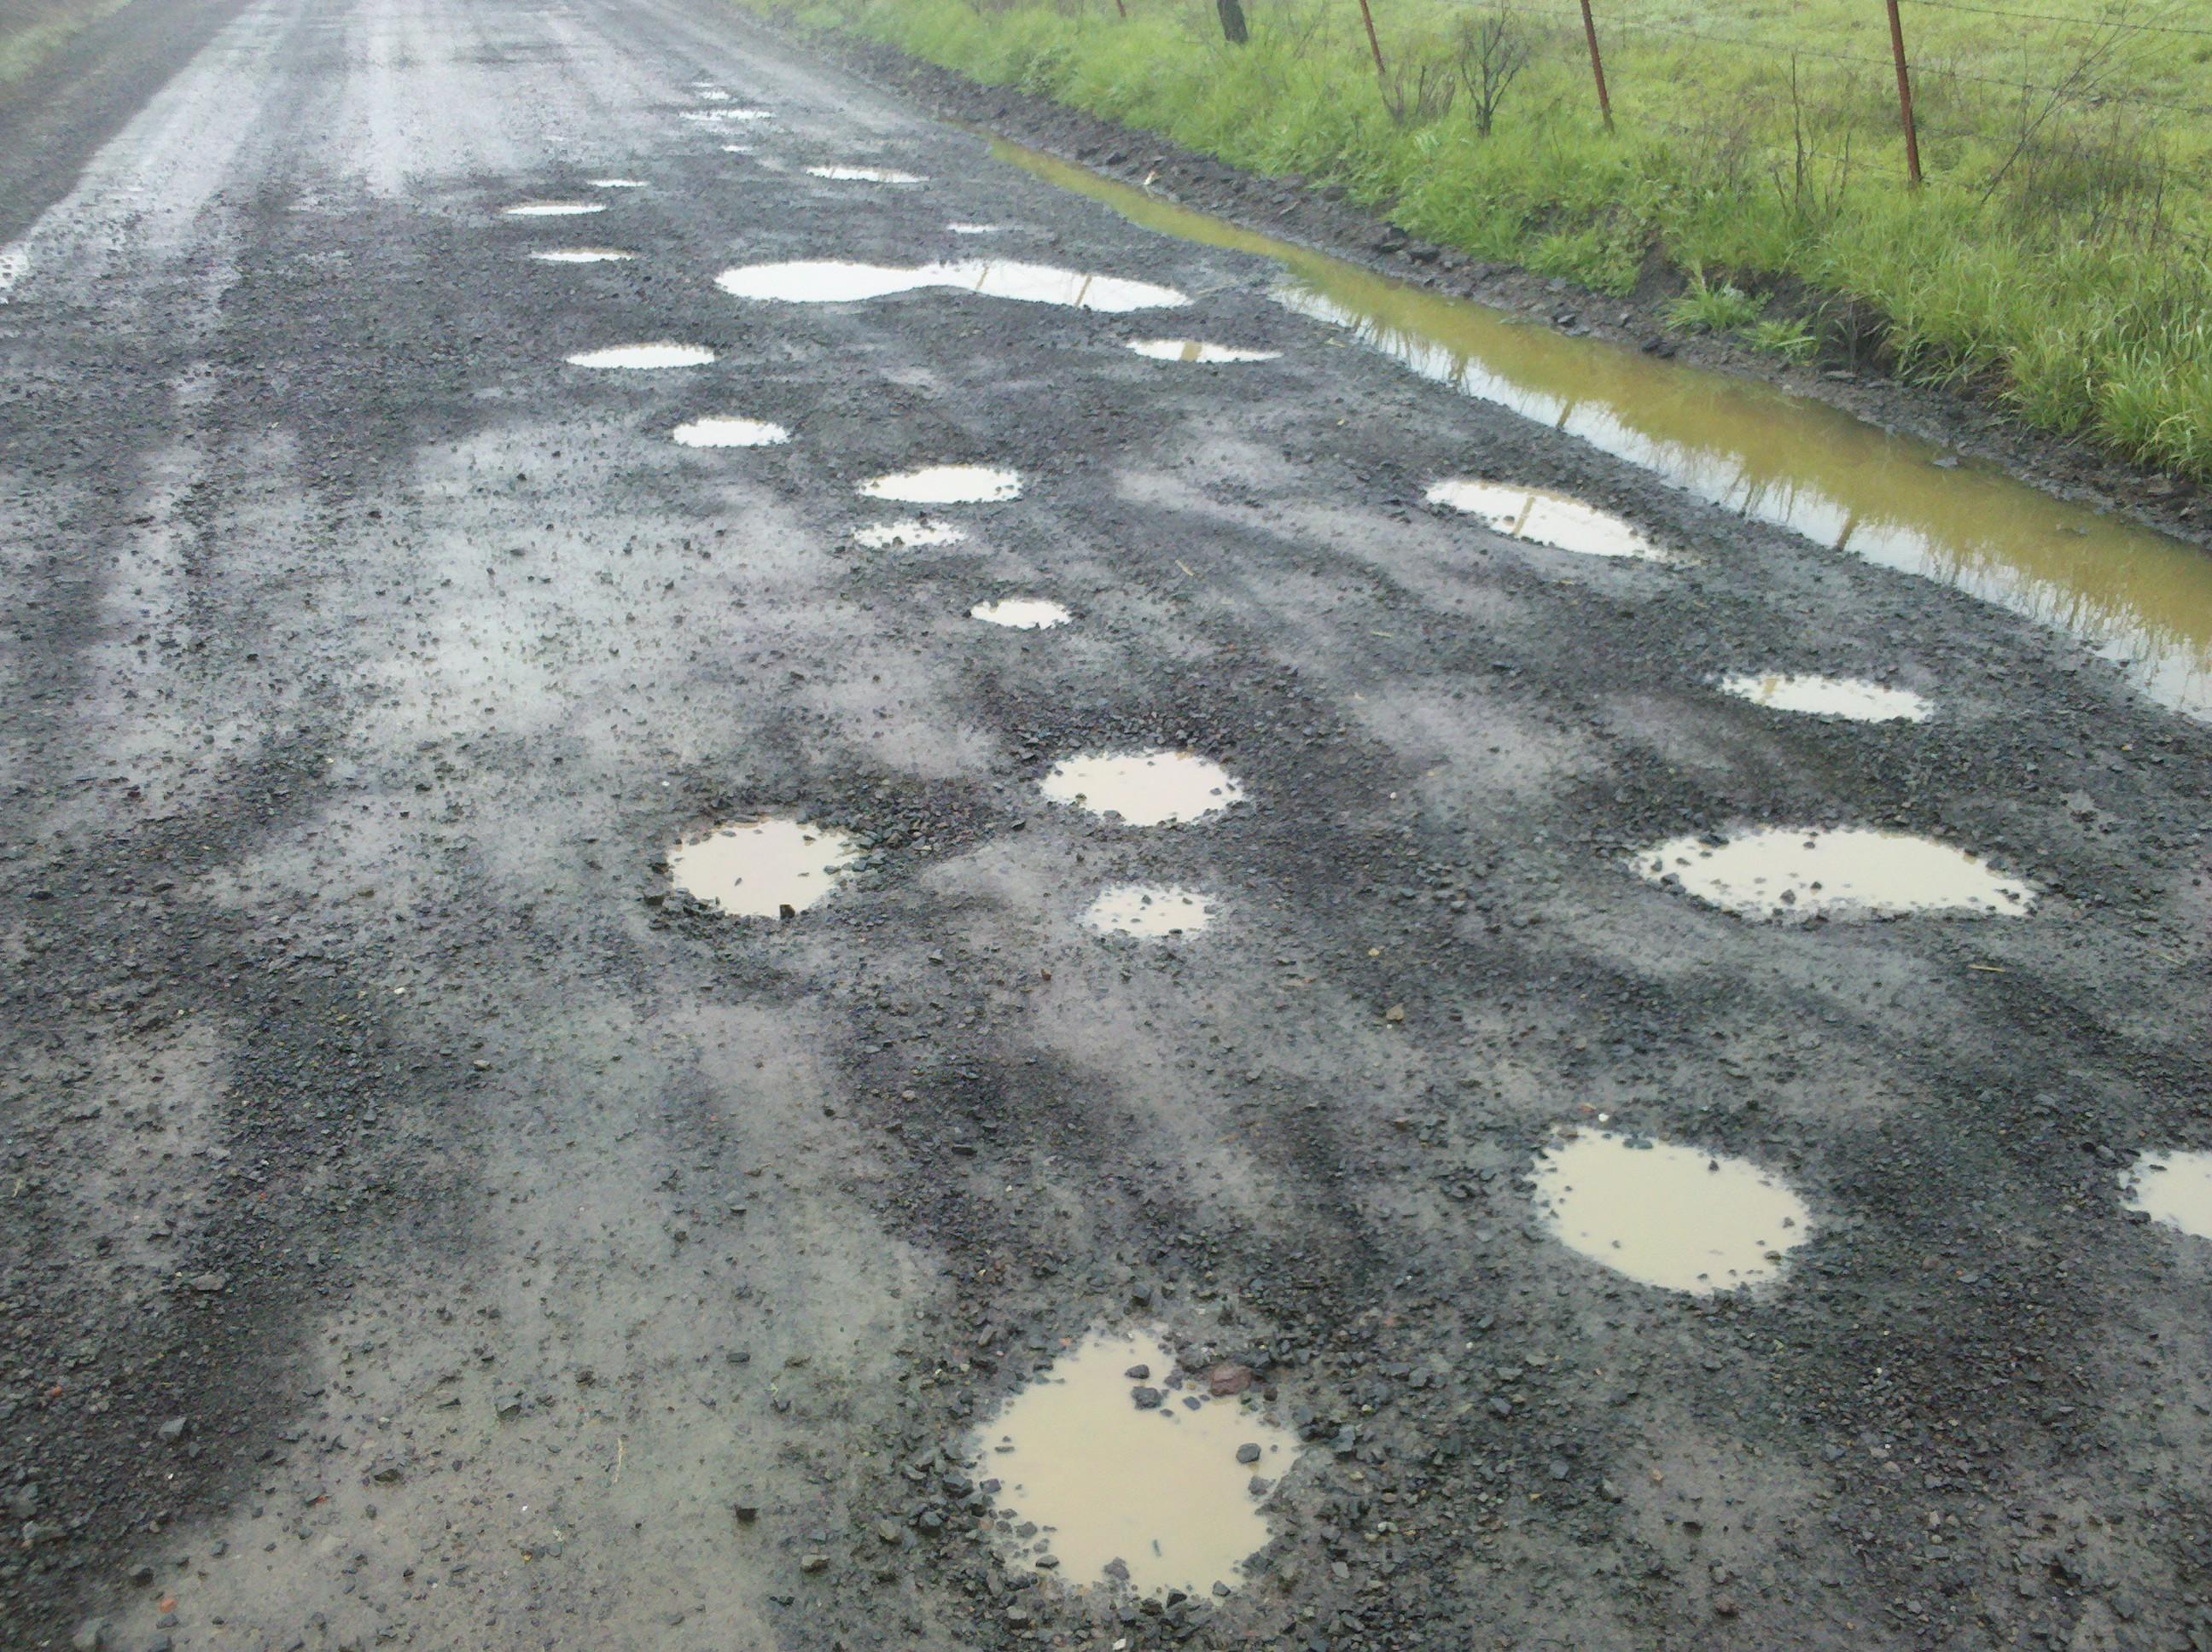
\includegraphics[width = 3in]{road_11}
        \caption{Original Image from the Google Images Dataset}
    \end{figure}

    \begin{figure}[ht!]
        \centering
        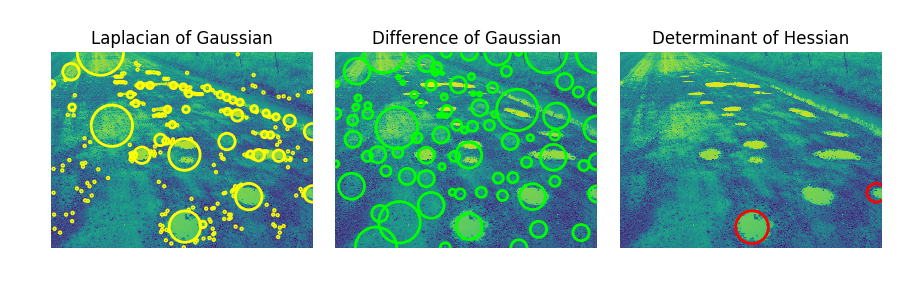
\includegraphics[width = 5in]{blob_3}
        \caption{Output of the three Blob Detection Techniques}
    \end{figure}
    
    \pagebreak
    
    \begin{figure}[ht!]
        \centering
        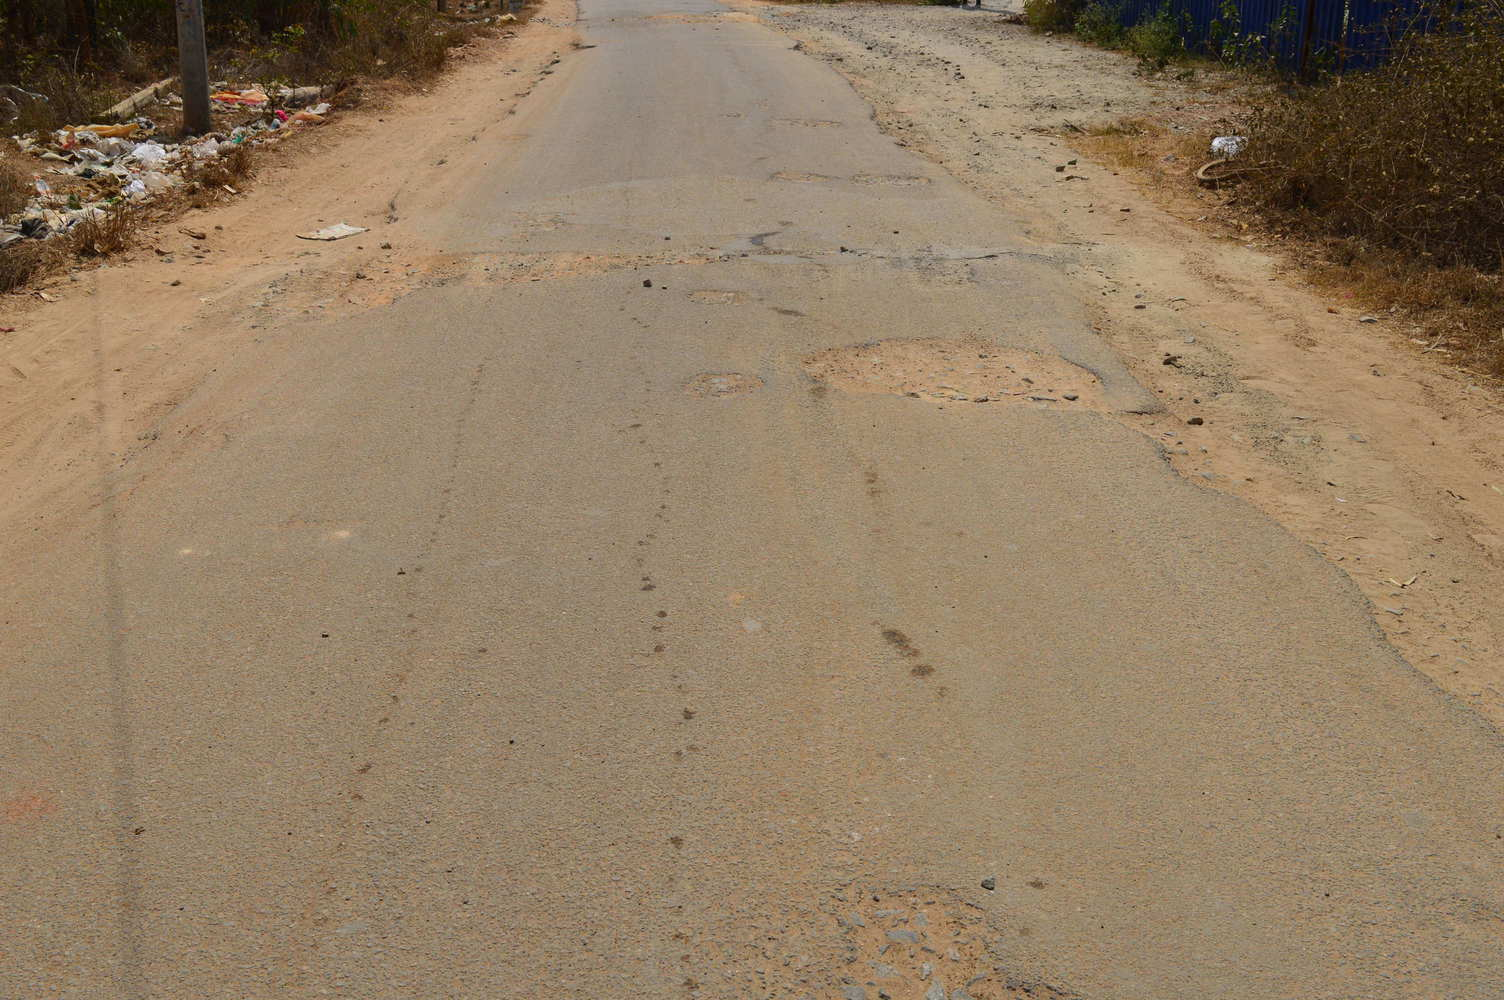
\includegraphics[width = 3in]{road_cam_8}
        \caption{Original Image from the Collected Dataset}
    \end{figure}
    
    \begin{figure}[ht!]
        \centering
        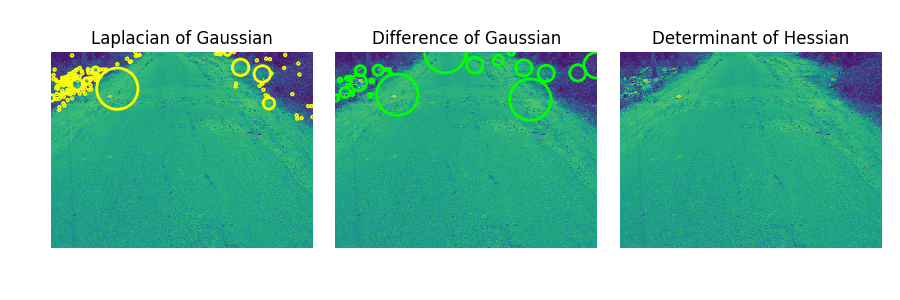
\includegraphics[width = 5in]{blob_1}
        \caption{Output of the three Blob Detection Techniques}
    \end{figure}
    
    \pagebreak
    \begin{figure}[ht!]
        \centering
        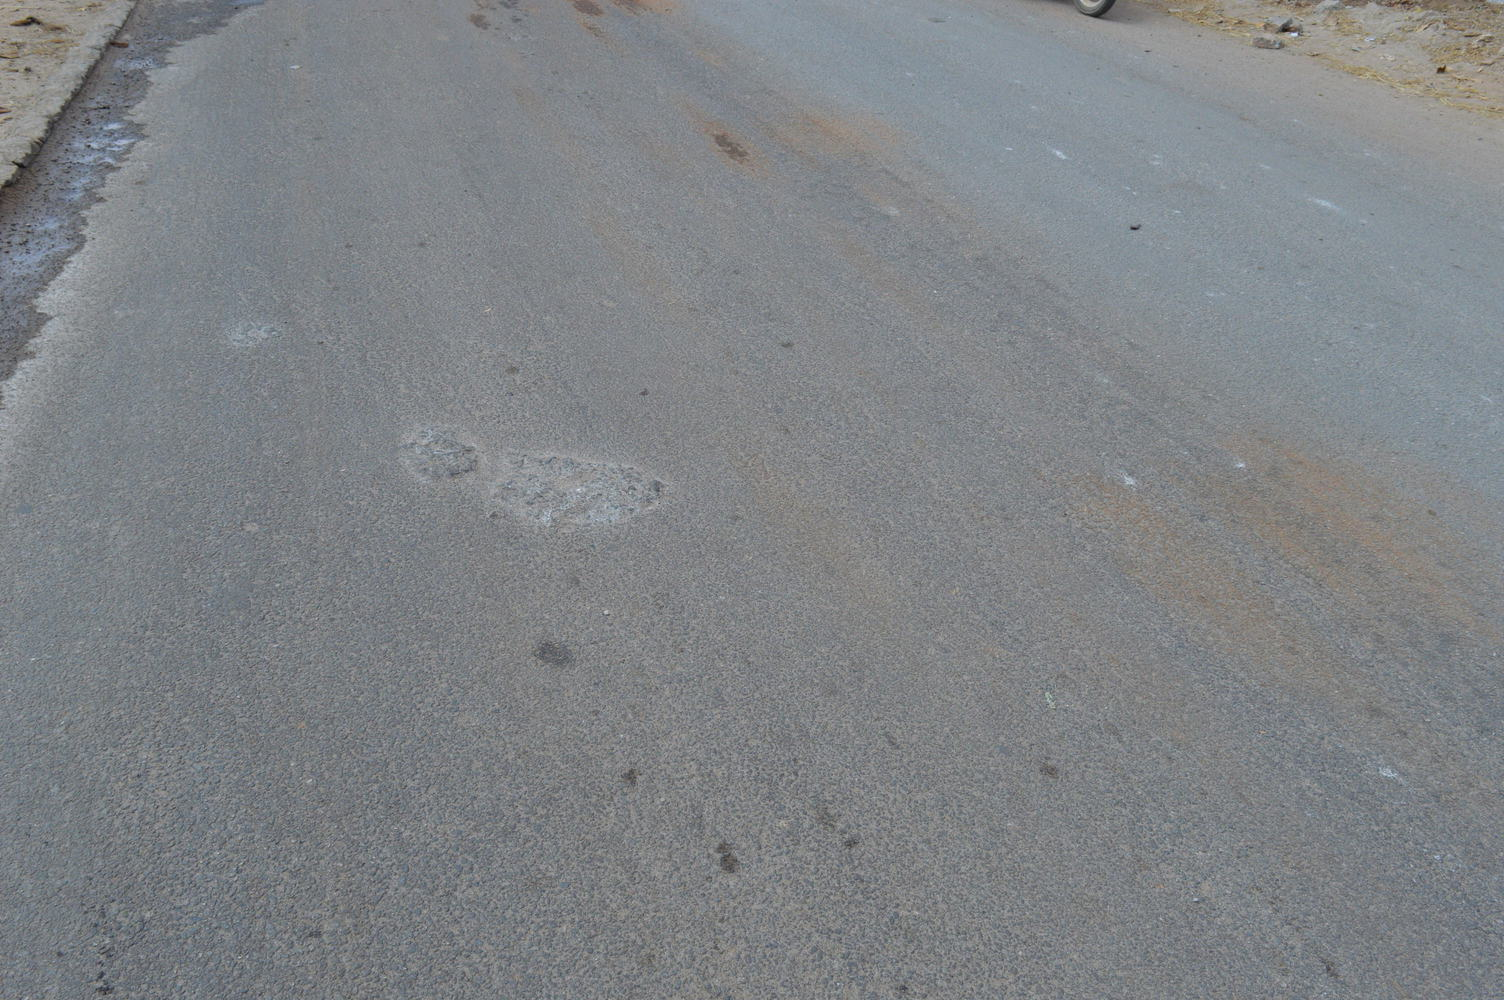
\includegraphics[width = 3in]{road_cam_3}
        \caption{Original Image from the Collected Dataset}
    \end{figure}

    \begin{figure}[ht!]
        \centering
        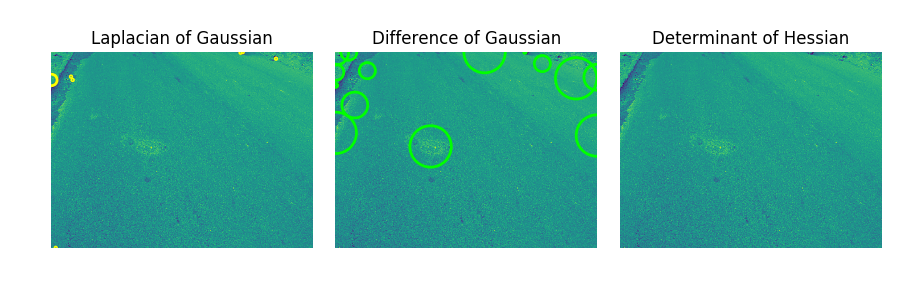
\includegraphics[width = 5in]{blob_2}
        \caption{Output of the three Blob Detection Techniques}
    \end{figure}
    \pagebreak
    
    \item \textbf{Method 2: Contour Detection with K-Means}
    \begin{enumerate}
        \item In the contour detection method with K-Means, we used the K-Means algorithm with 30 iterations and 3 clusters. The Gaussian Blur was applied to the output of the K-Means to remove any noise in the frames. Finally, the Canny Edge Detection algorithm was used to find out the edges and contours around potholes in the frames. This technique detected potholes and some of the noise in the Google Images dataset but it did not work with our dataset. It missed the contours for potholes and detected shadows in some of the frames.
    \end{enumerate}
    \pagebreak
    
    \begin{figure}[ht!]
        \centering
        \includegraphics[width = 3in]{road_7}
        \caption{Original Image from the Google Images Dataset}
    \end{figure}

    \begin{figure}[ht!]
        \centering
        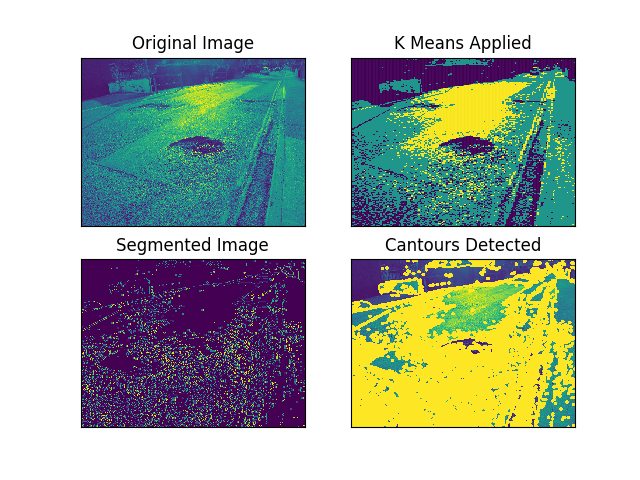
\includegraphics[width = 5in]{kmeans_1}
        \caption{Output of Contour Detection using K-Means}
    \end{figure}
    \pagebreak
    
    \begin{figure}[ht!]
        \centering
        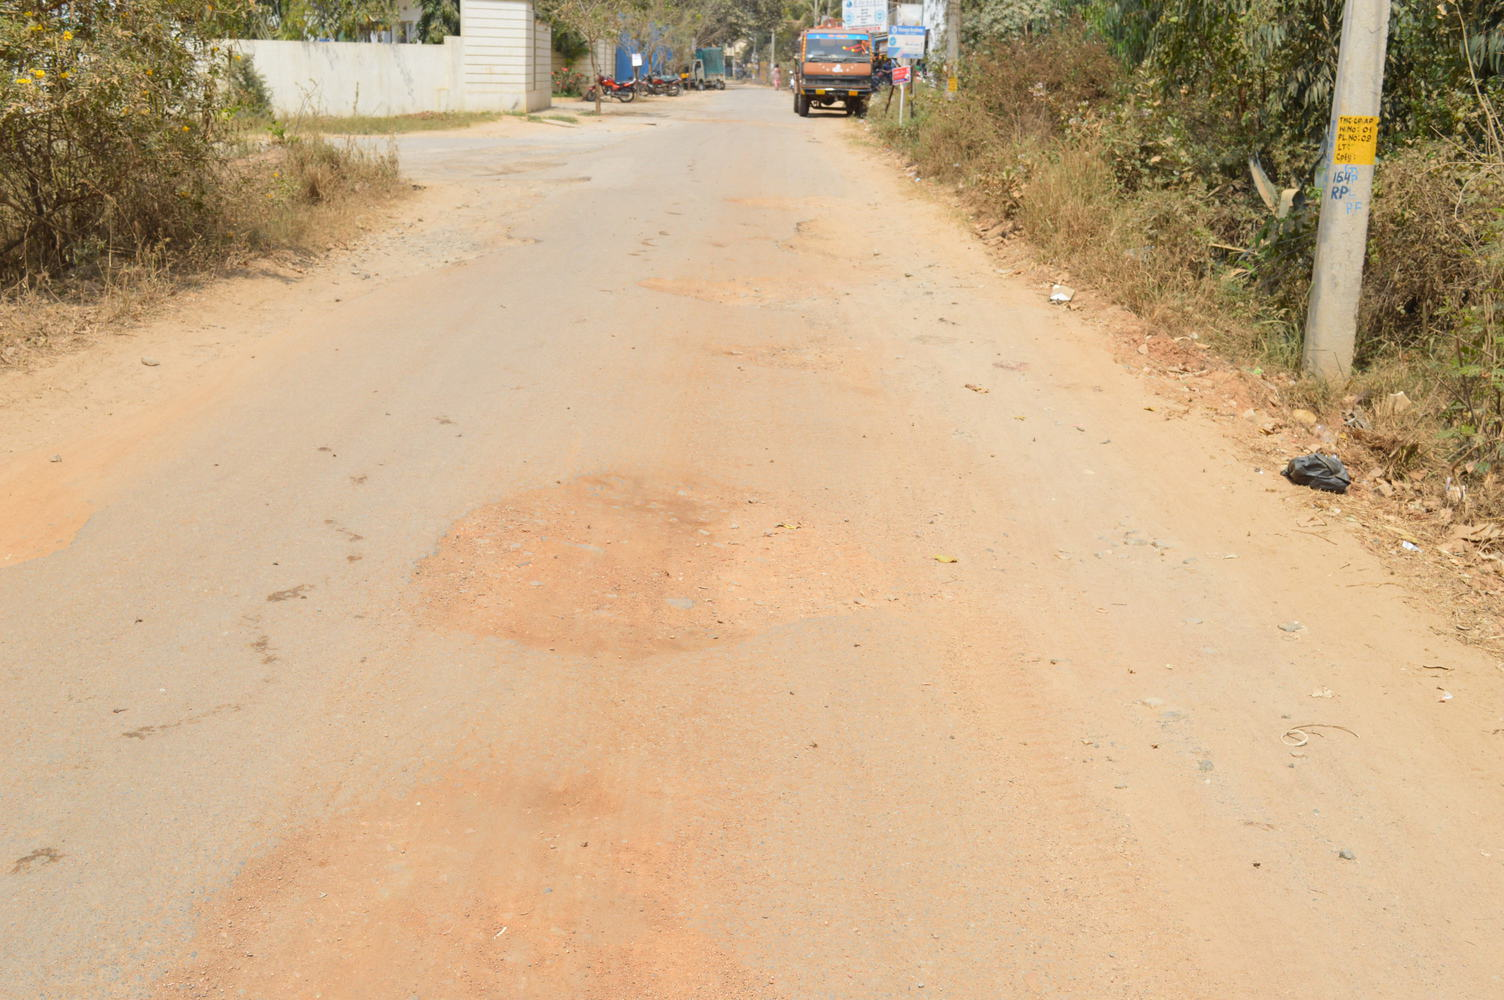
\includegraphics[width = 3in]{road_cam_14}
        \caption{Original Image from the Collected Dataset}
    \end{figure}

    \begin{figure}[ht!]
        \centering
        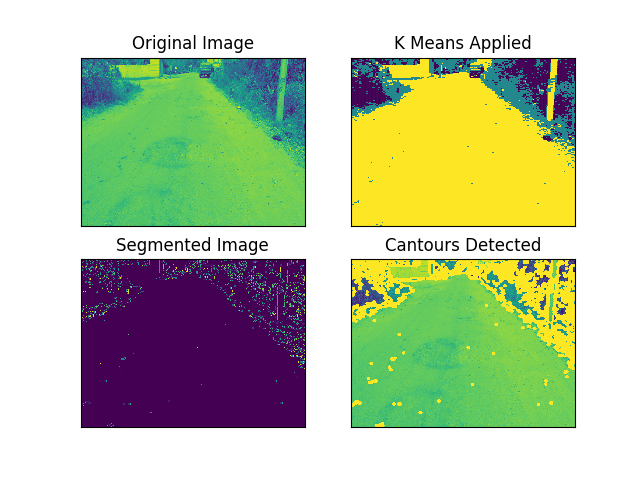
\includegraphics[width = 5in]{kmeans_2}
        \caption{Output of Contour Detection using K-Means}
    \end{figure}
    \pagebreak
    
    \begin{figure}[ht!]
        \centering
        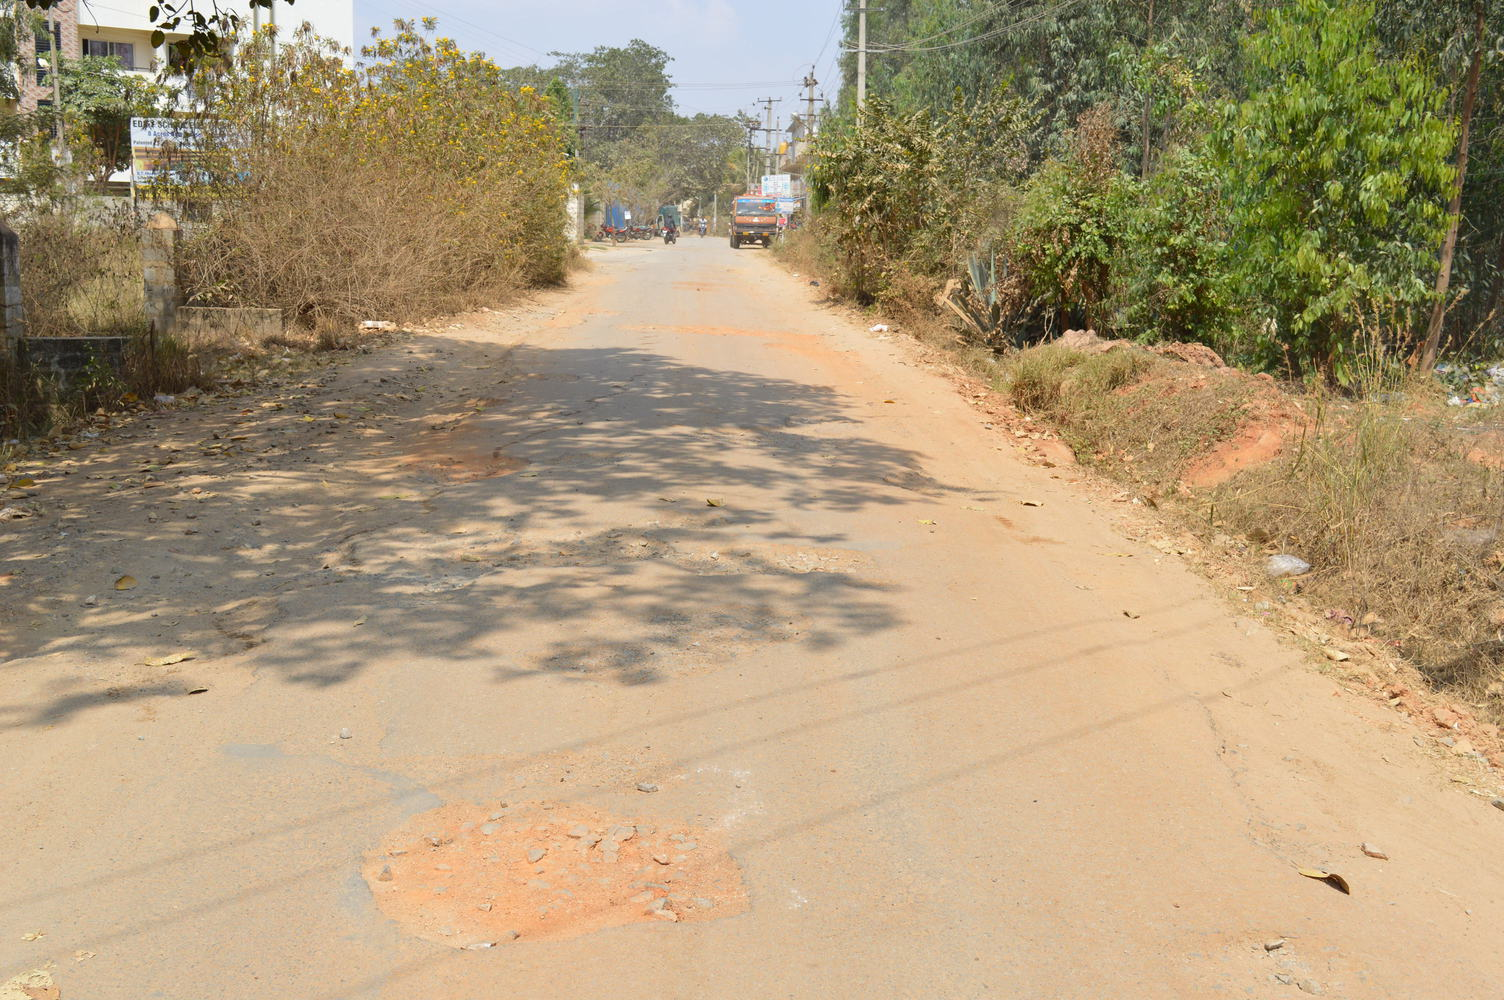
\includegraphics[width = 3in]{road_cam_11}
        \caption{Original Image from the Collected Dataset}
    \end{figure}

    \begin{figure}[ht!]
        \centering
        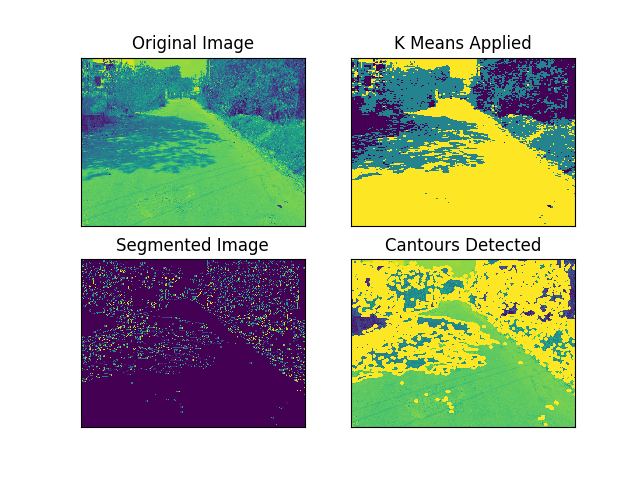
\includegraphics[width = 5in]{kmeans_3}
        \caption{Output of Contour Detection using K-Means}
    \end{figure}
    \pagebreak
    
    \item \textbf{Method 3:Contour Detection with Meanshift}
    \begin{enumerate}
        \item Using the idea of the previous methodology of Contour Detection, we used Meanshift as the clustering algorithm instead of the K-means algorithm. The inbuilt function \textbf{pyrMeanShiftFiltering} was used to filter and segment the image with arguments \textbf{Spatial Window Radius} as 25, \textbf{Color Window Radius} as 45 and \textbf{Maximum Level Of Segmentation} as 10. Similar to the previous methodology, Gaussian Blur and Canny Edge Detection were applied to find the contours in the frames.This method worked perfectly on the Google Images Dataset but detected the potholes partially in our dataset with the additional noise.
    \end{enumerate}
    \pagebreak
    
    \begin{figure}[ht!]
        \centering
        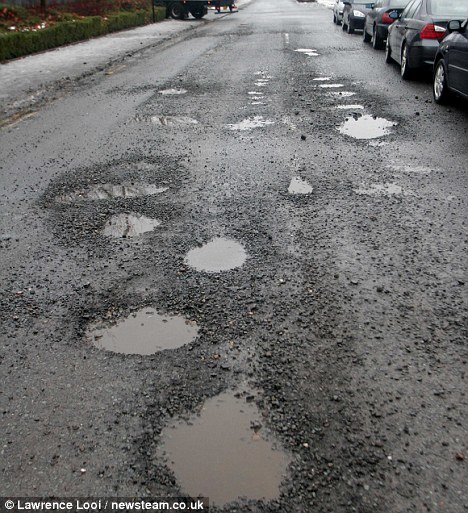
\includegraphics[width = 2in]{road_10}
        \caption{Original Image from the Google Images Dataset}
    \end{figure}

    \begin{figure}[ht!]
        \centering
        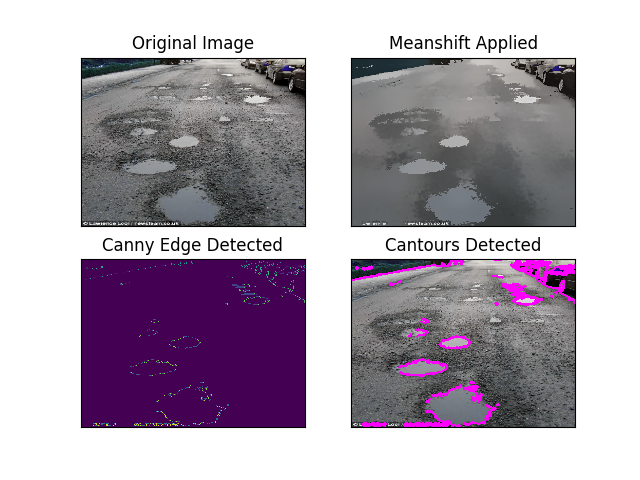
\includegraphics[width = 5in]{meanshift_2}
        \caption{Output of Contour Detection using Meanshift}
    \end{figure}
    \pagebreak
    
    \begin{figure}[ht!]
        \centering
        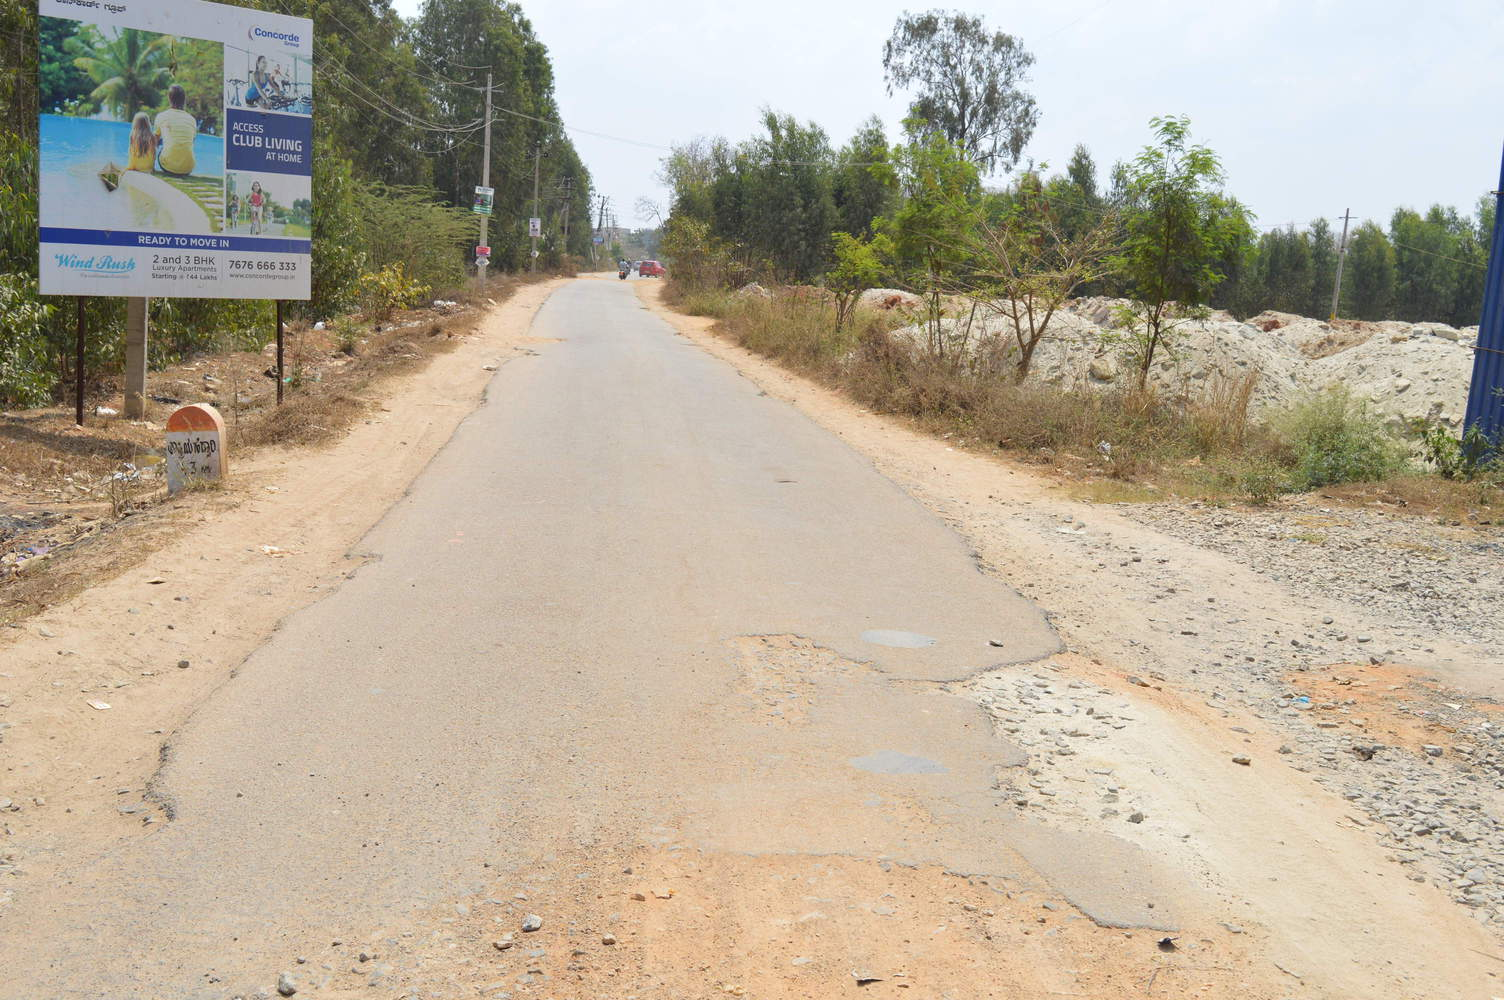
\includegraphics[width = 3in]{road_cam_25}
        \caption{Original Image from the Collected Dataset}
    \end{figure}

    \begin{figure}[ht!]
        \centering
        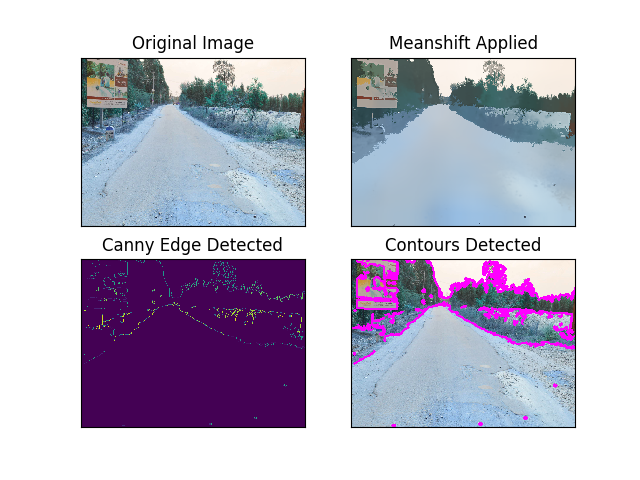
\includegraphics[width = 5in]{meanshift_1}
        \caption{Output of Contour Detection using Meanshift}
    \end{figure}
    \pagebreak

    
    \begin{figure}[ht!]
        \centering
        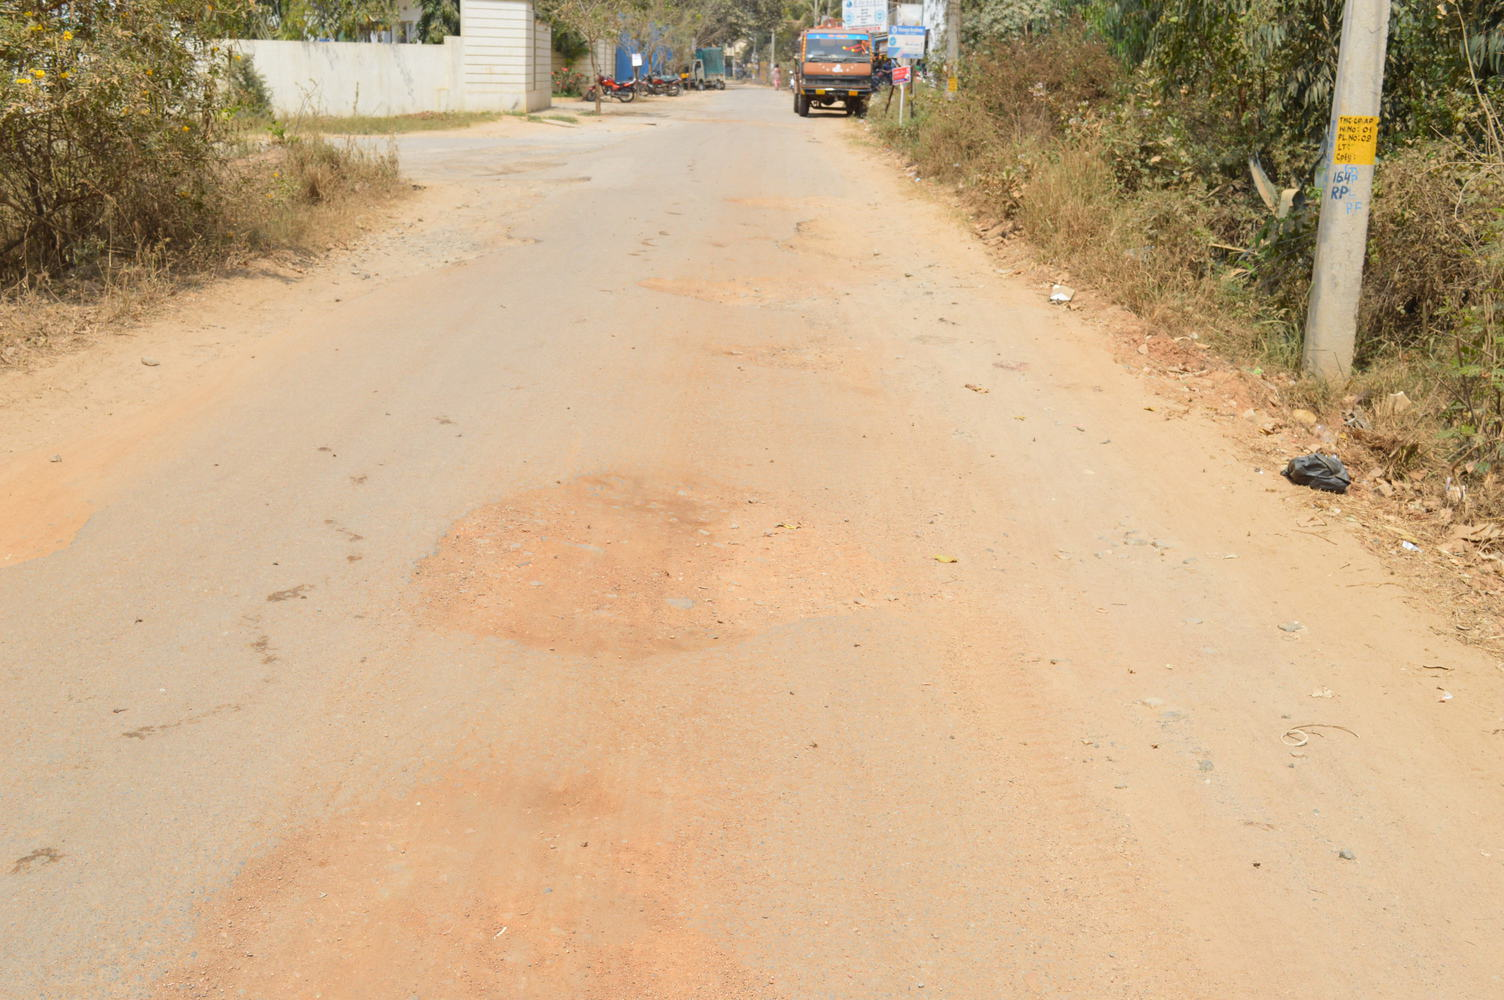
\includegraphics[width = 3in]{road_cam_14}
        \caption{Original Image from the Collected Dataset}
    \end{figure}

    \begin{figure}[ht!]
        \centering
        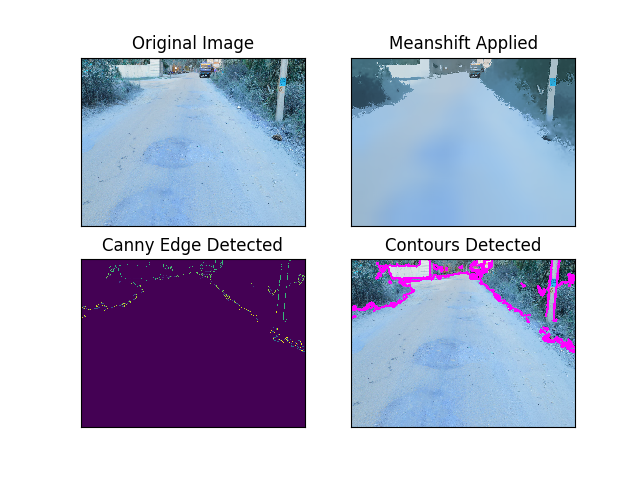
\includegraphics[width = 5in]{meanshift_3}
        \caption{Output of Contour Detection using Meanshift}
    \end{figure}
    \pagebreak
    
    \begin{figure}[ht!]
        \centering
        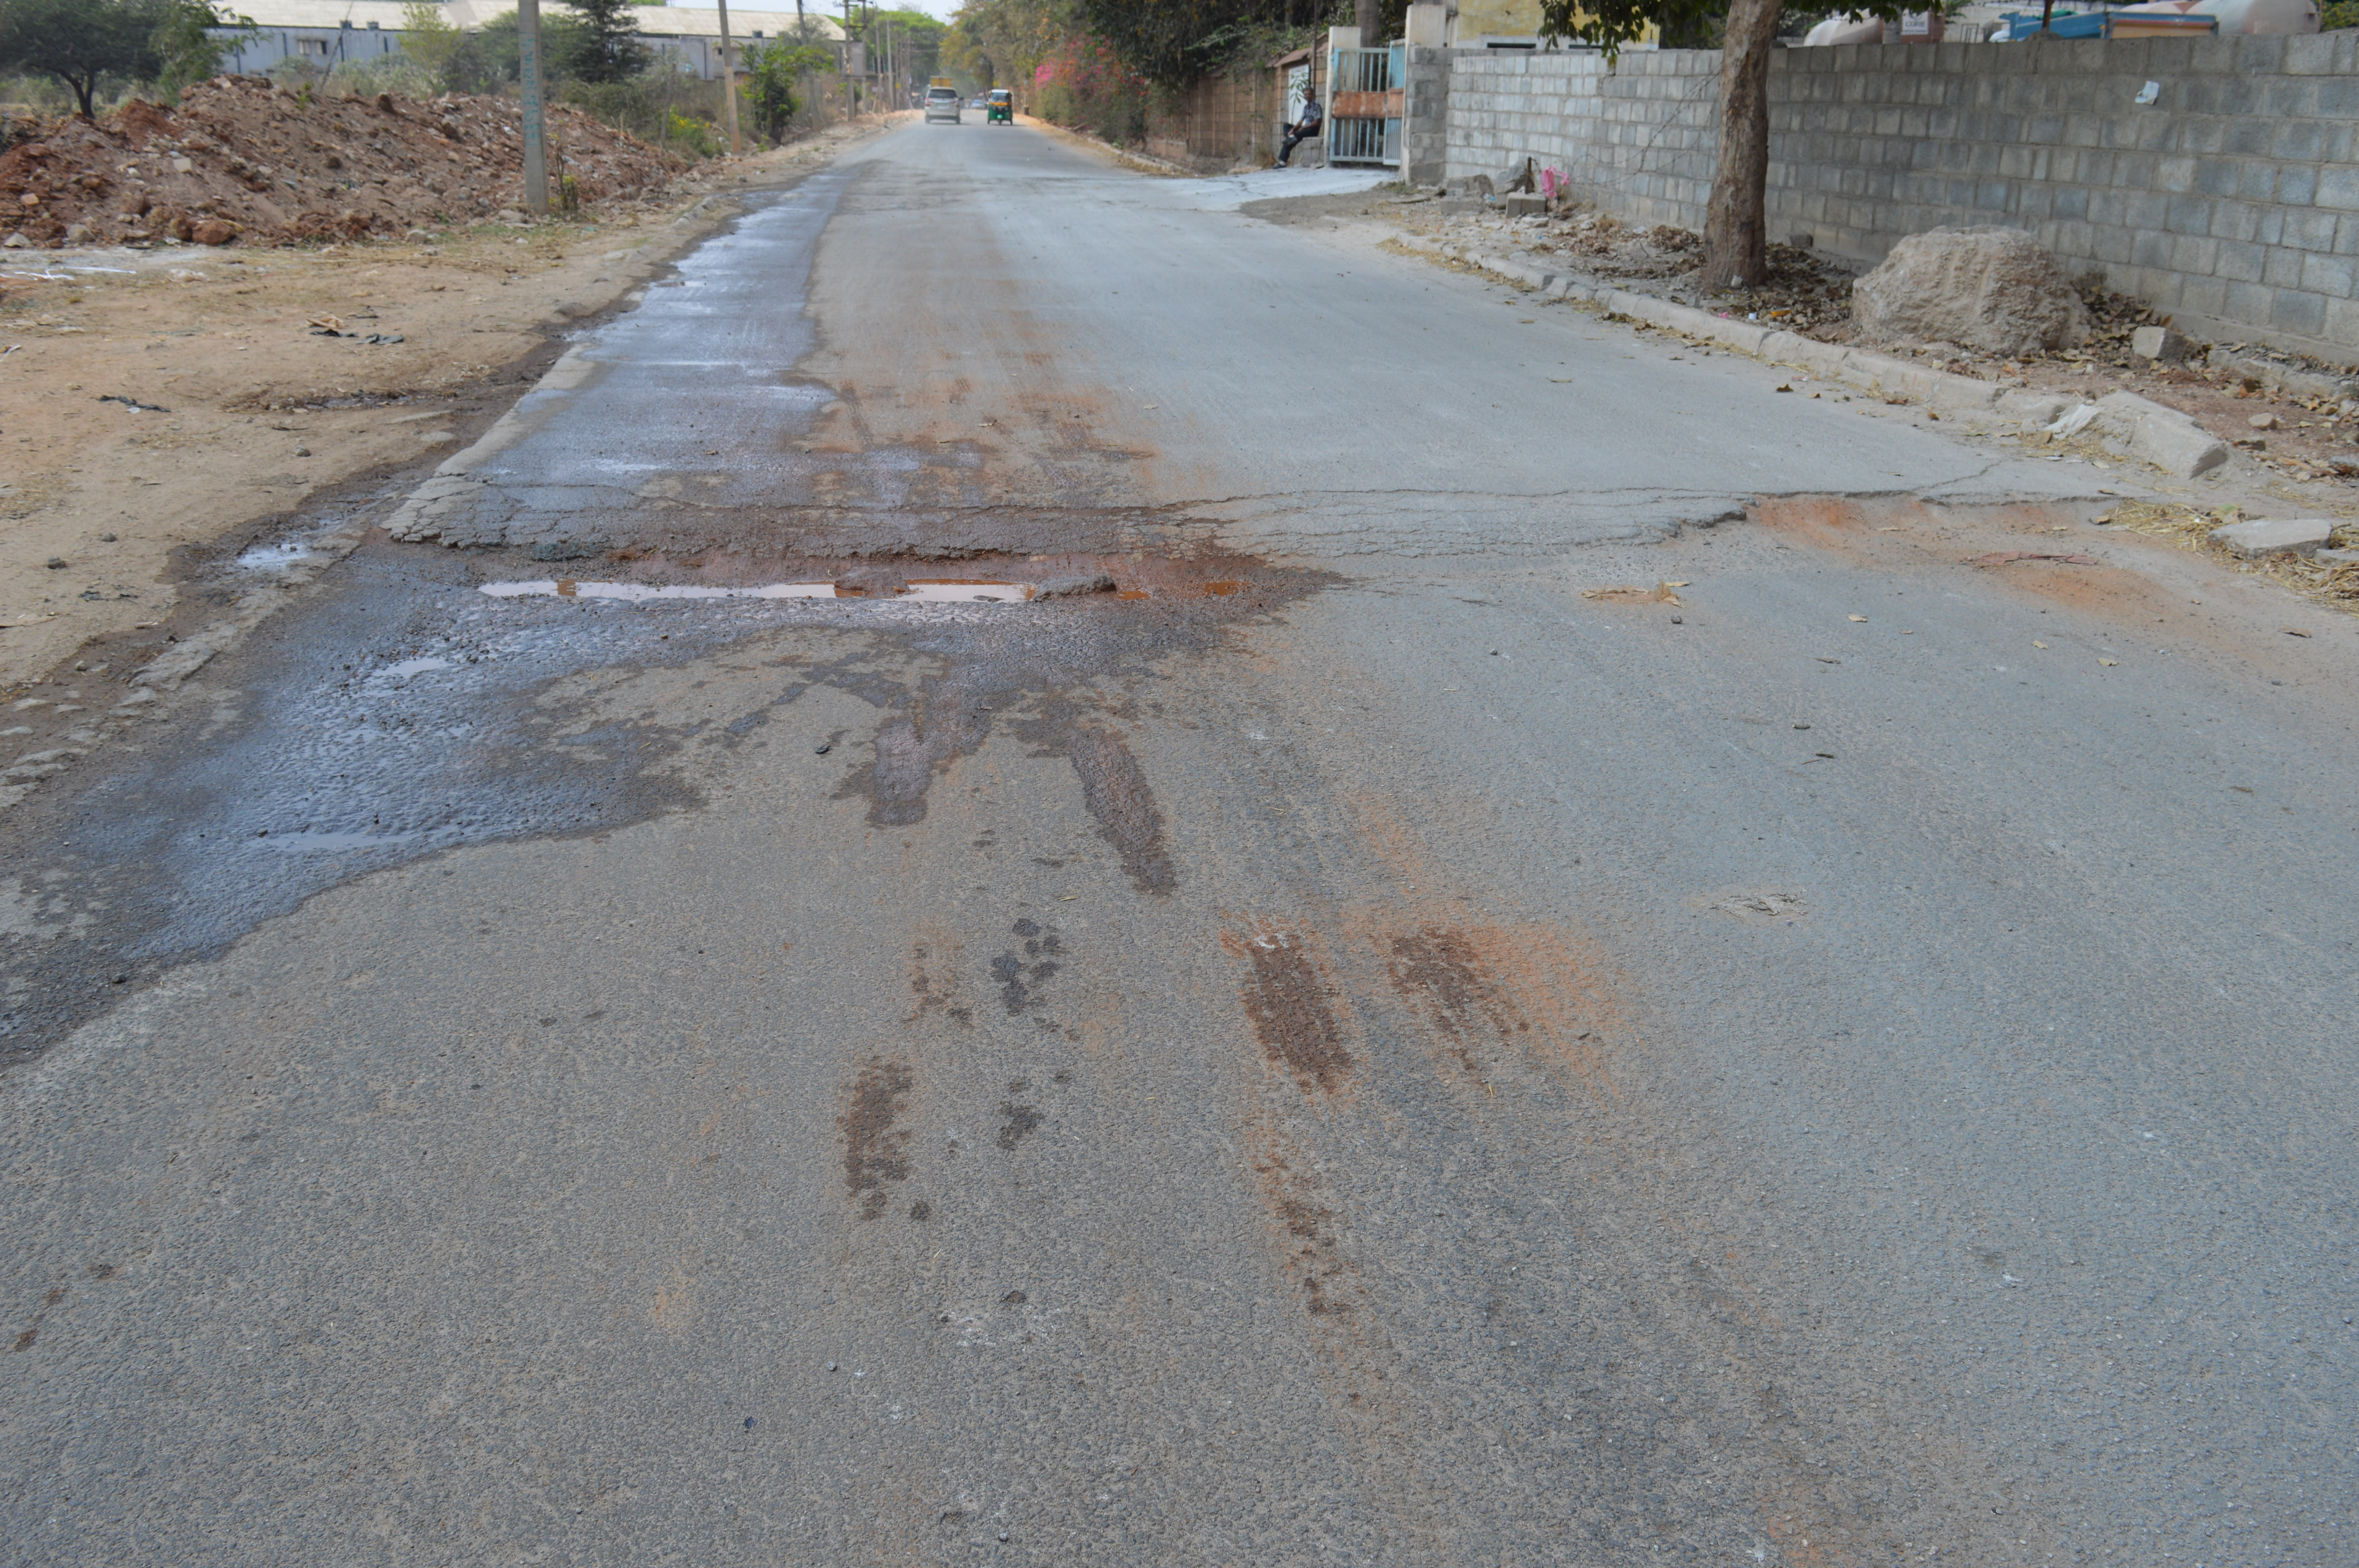
\includegraphics[width = 3in]{DSC_2524}
        \caption{Original Image from the Collected Dataset}
    \end{figure}

    \begin{figure}[ht!]
        \centering
        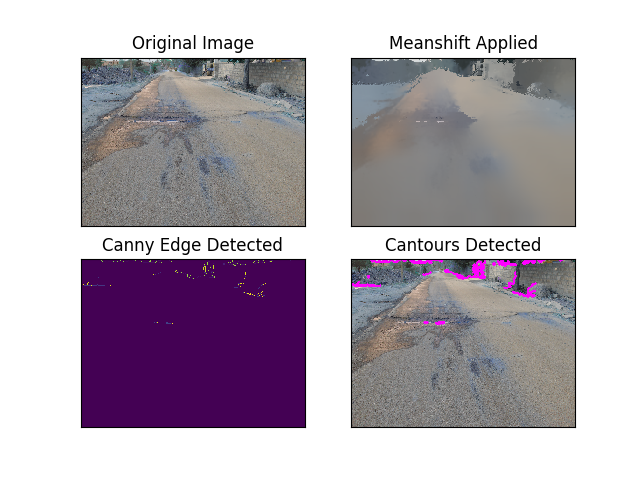
\includegraphics[width = 5in]{meanshift_4}
        \caption{Output of Contour Detection using Meanshift}
    \end{figure}
    \pagebreak
    
    \item \textbf{Method 4: Contour Detection with Morphological Transformation}
    \begin{enumerate}
        \item In the Contour Detection method with Morphological Transformations, we used erosion to detect contours around potholes in the images. Gaussian Blur and thresholding was applied on the input frames to remove the noise signals from the image. The results of Image Gradients: Laplacian, Sobel X, Sobel Y were compared, after applying them on the blurred image. Among all, Sobel Y, performed the best. Then, erosion was applied to this output frame, with the medium sized kernel, to narrow down the search for potholes in the frames. Contours were being detected in the final frame. This technique worked on the Google Images dataset with partial noise being detected but detected too much noise in our dataset alongwith a fraction of potholes.
    \end{enumerate}
    \begin{figure}[ht!]
        \centering
        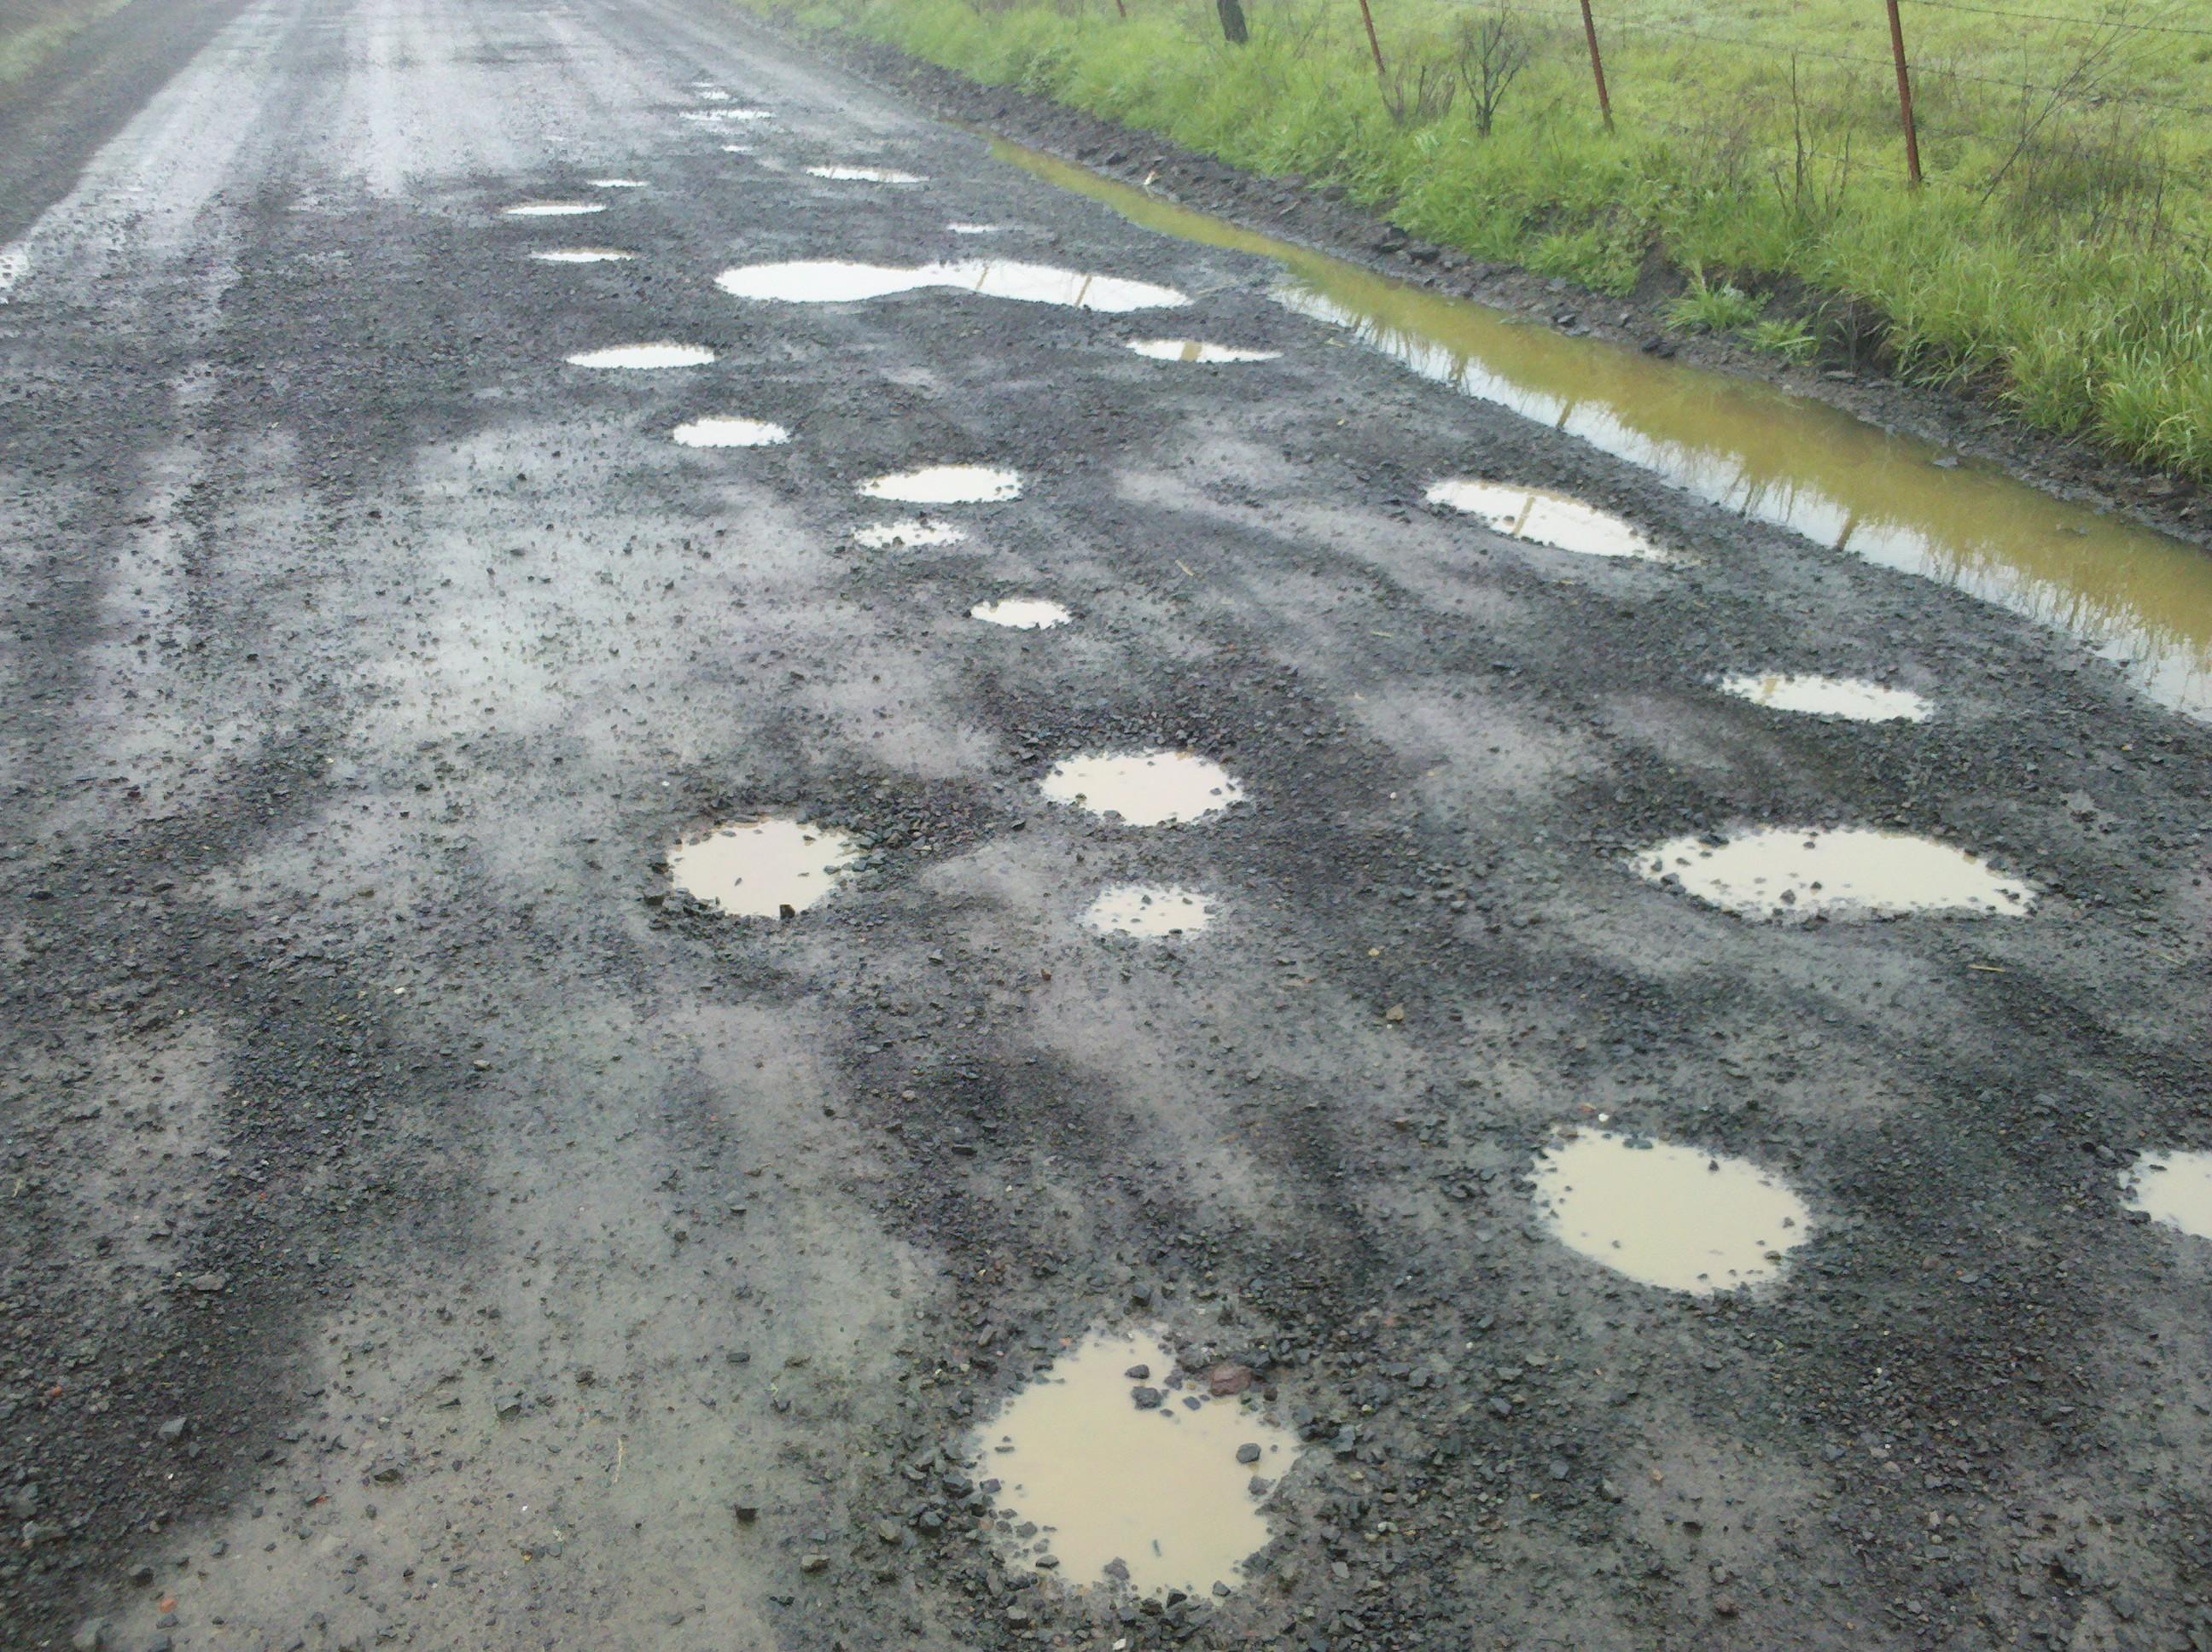
\includegraphics[width = 3in]{road_11}
        \caption{Original Image from the Google Images Dataset}
    \end{figure}

    \begin{figure}[ht!]
        \centering
        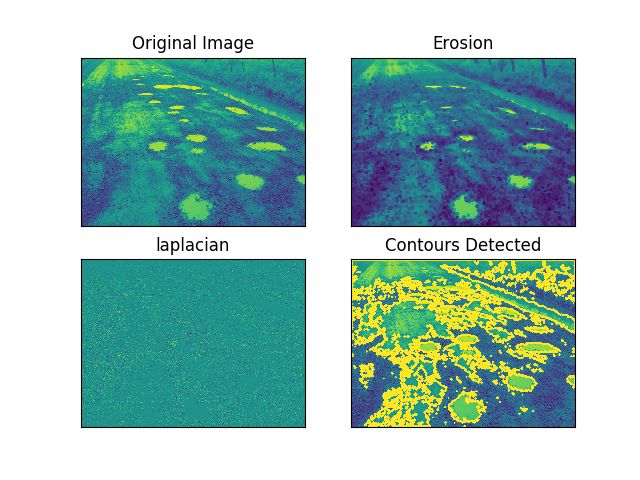
\includegraphics[width = 5in]{morph_transform_2}
        \caption{Output of Contour Detection using Morphological Transformation}
    \end{figure}
    \pagebreak
    
    \begin{figure}[ht!]
        \centering
        \includegraphics[width = 3in]{road_7}
        \caption{Original Image from the Google Images Dataset}
    \end{figure}

    \begin{figure}[ht!]
        \centering
        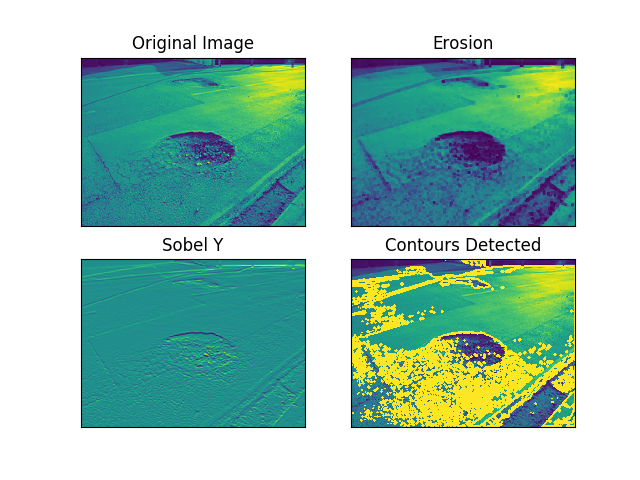
\includegraphics[width = 5in]{morph_transform_6}
        \caption{Output of Contour Detection using Morphological Transformation}
    \end{figure}
    \pagebreak
    
    \begin{figure}[ht!]
        \centering
        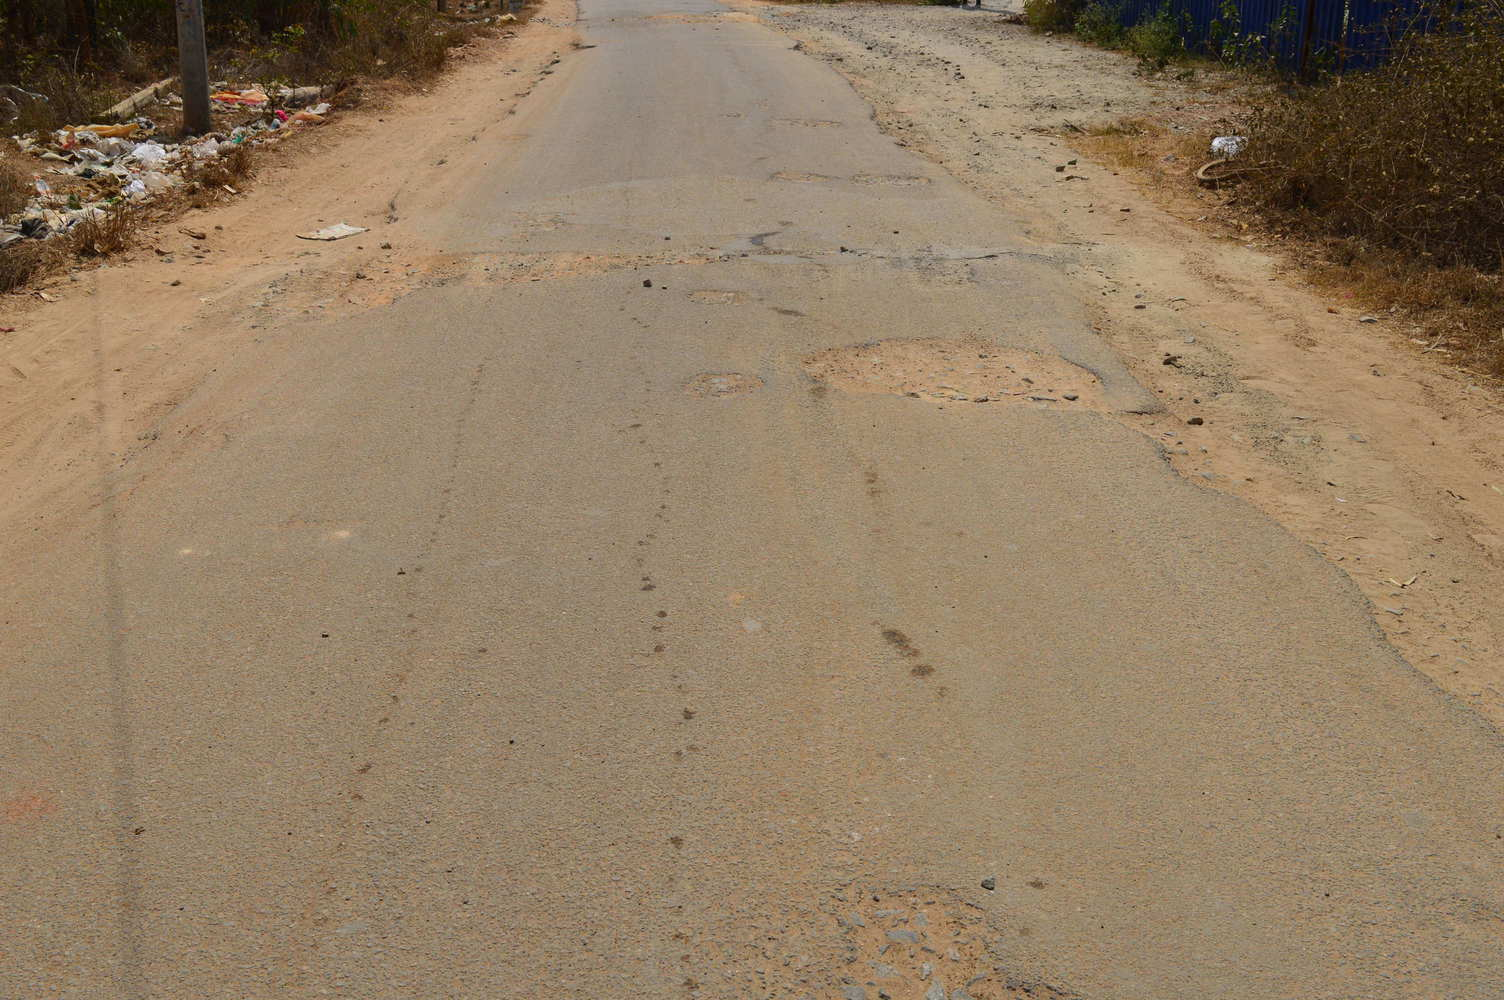
\includegraphics[width = 3in]{road_cam_8}
        \caption{Original Image from the Collected Dataset}
    \end{figure}

    \begin{figure}[ht!]
        \centering
        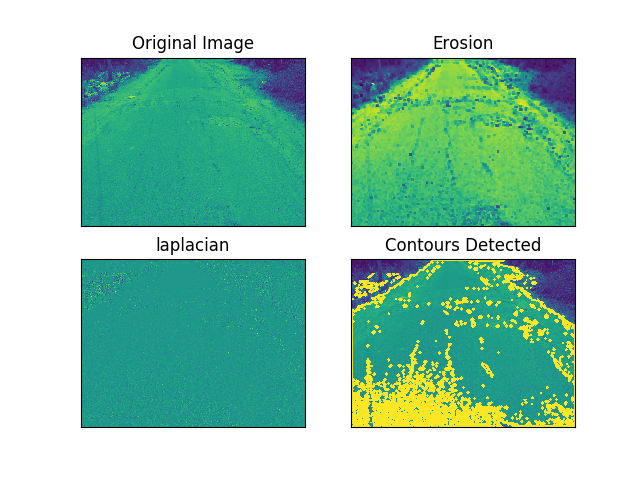
\includegraphics[width = 5in]{morph_transform_3}
        \caption{Output of Contour Detection using Morphological Transformation}
    \end{figure}
    \pagebreak
    
    \begin{figure}[ht!]
        \centering
        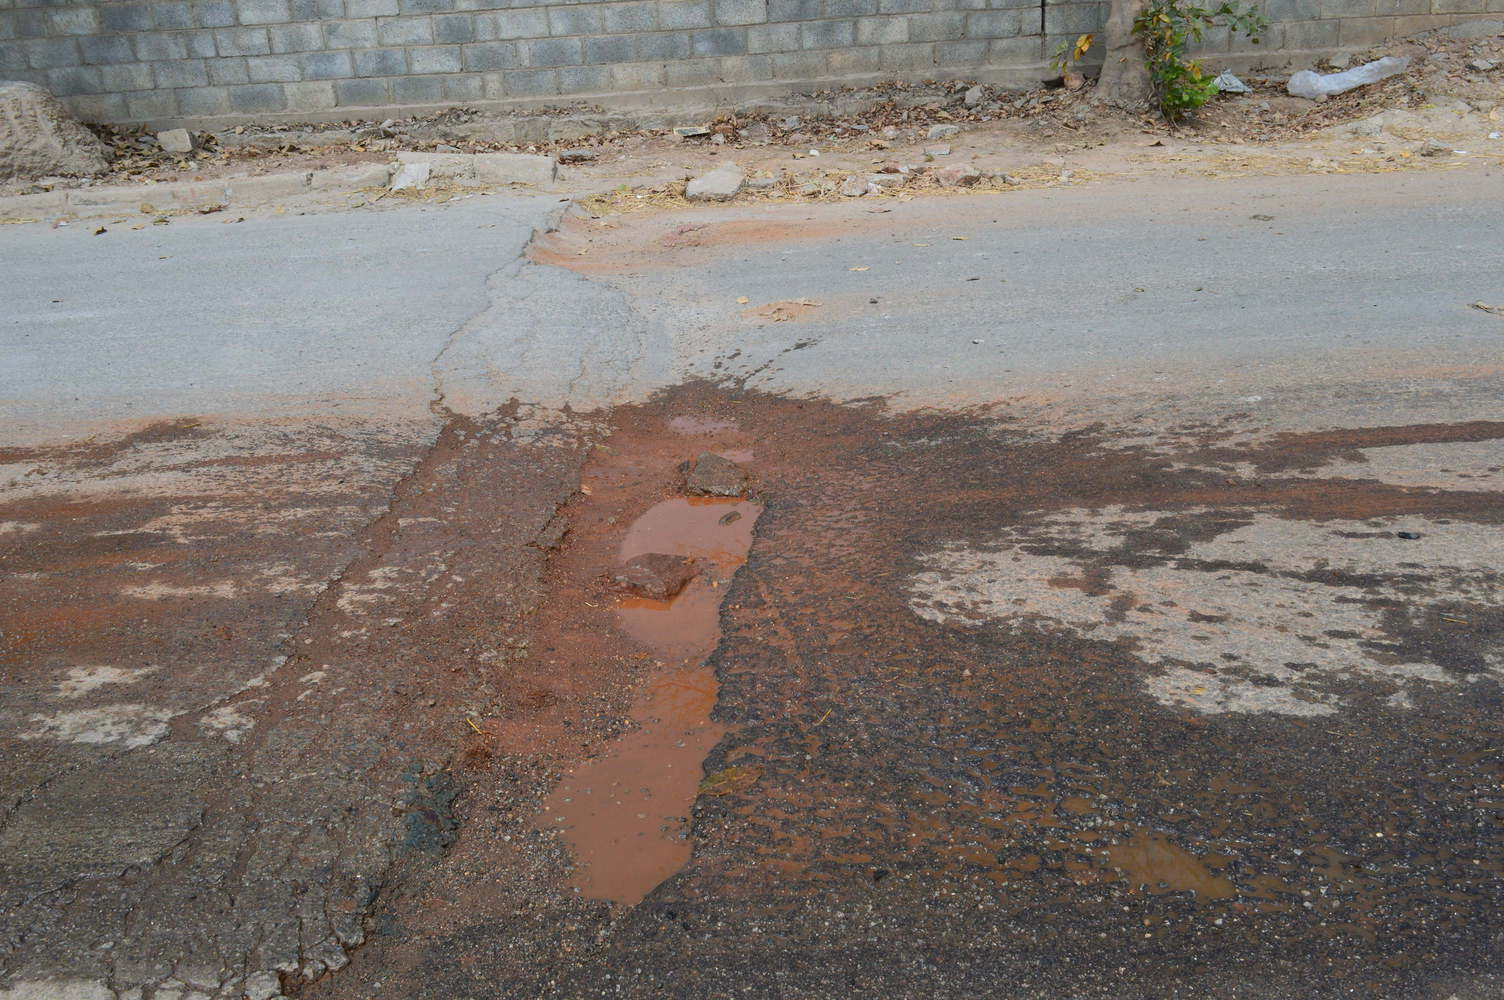
\includegraphics[width = 3in]{road_cam_2}
        \caption{Original Image from the Collected Dataset}
    \end{figure}

    \begin{figure}[ht!]
        \centering
        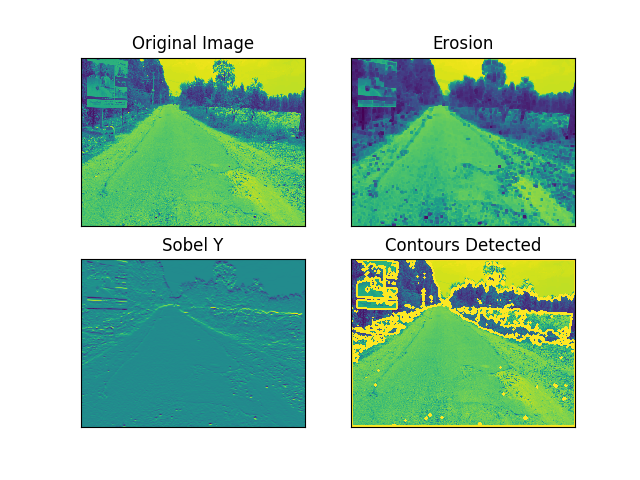
\includegraphics[width = 5in]{morph_transform_4}
        \caption{Output of Contour Detection using Morphological Transformation}
    \end{figure}
    \pagebreak
    
    \begin{figure}[ht!]
        \centering
        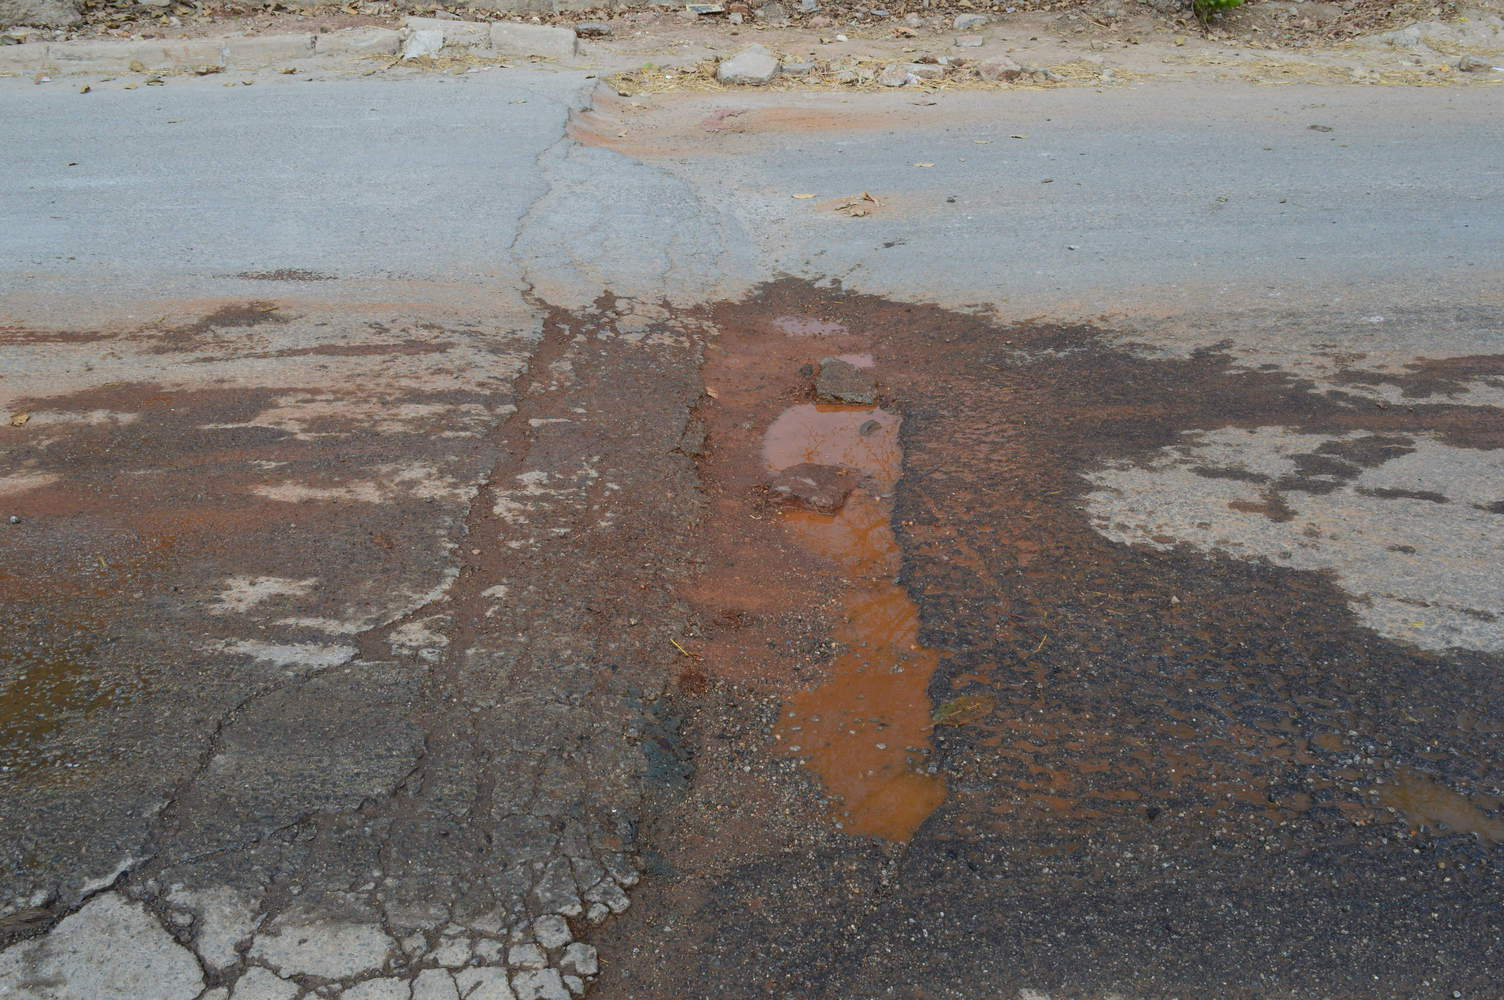
\includegraphics[width = 3in]{road_cam_6}
        \caption{Original Image from the Collected Dataset}
    \end{figure}

    \begin{figure}[ht!]
        \centering
        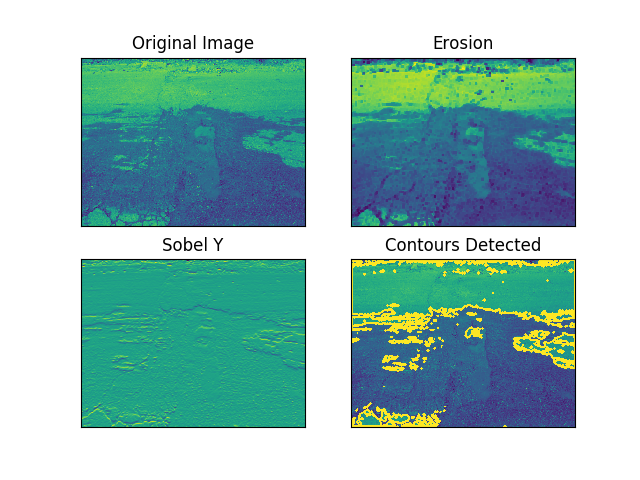
\includegraphics[width = 5in]{morph_transform_5}
        \caption{Output of Contour Detection using Morphological Transformation}
    \end{figure}
    \pagebreak
    
    \begin{figure}[ht!]
        \centering
        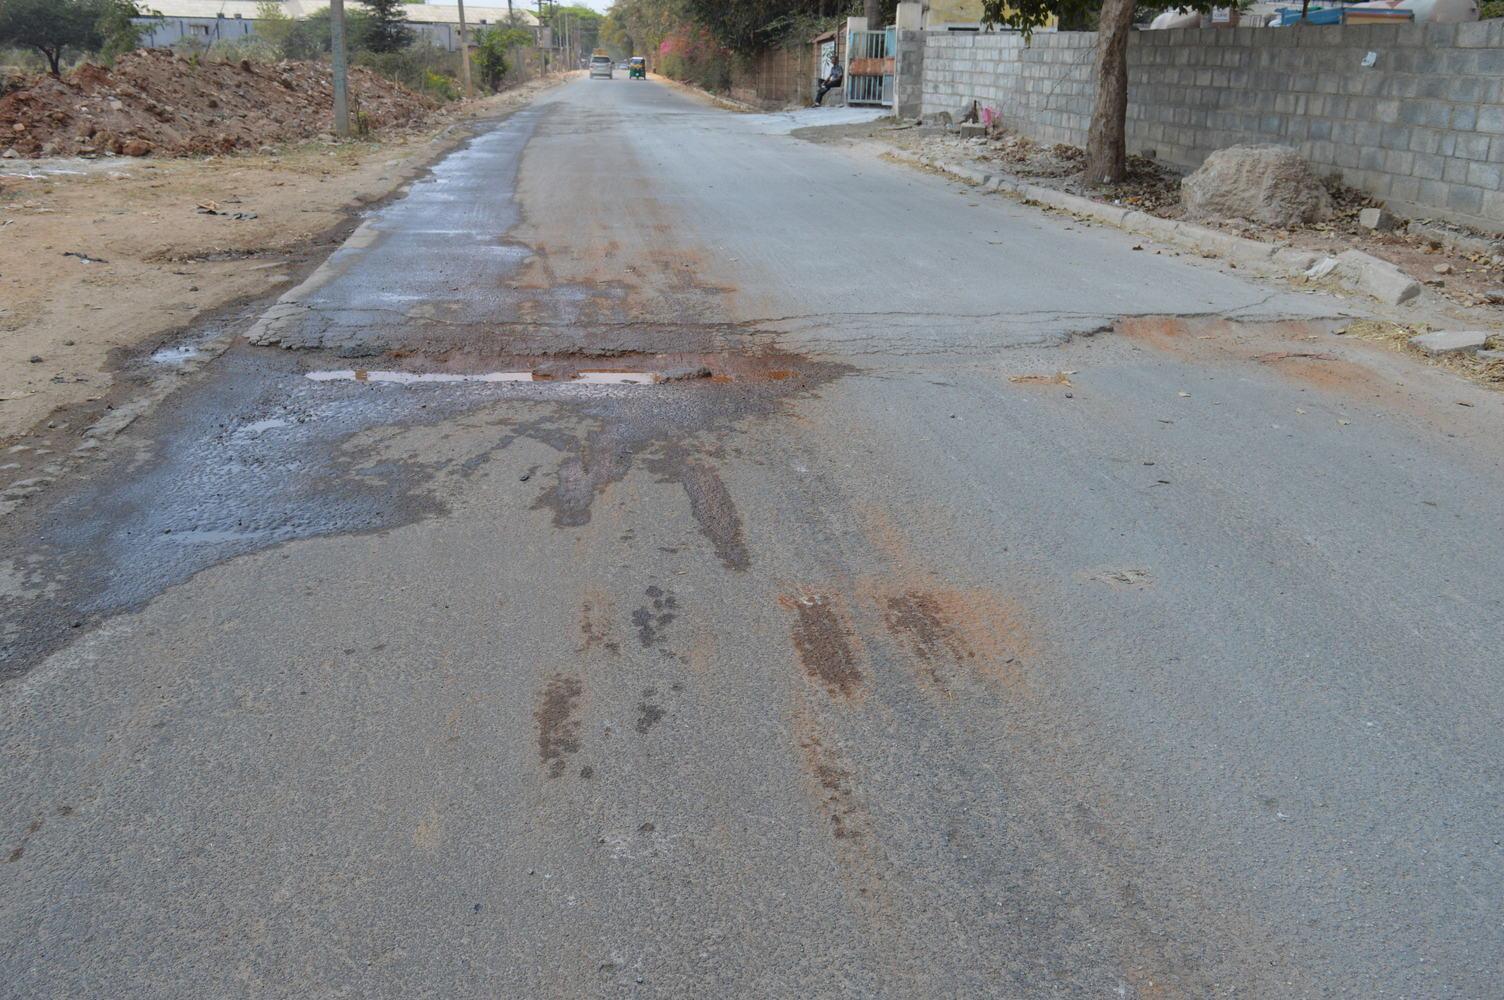
\includegraphics[width = 3in]{road_cam_4}
        \caption{Original Image from the Collected Dataset}
    \end{figure}

    \begin{figure}[ht!]
        \centering
        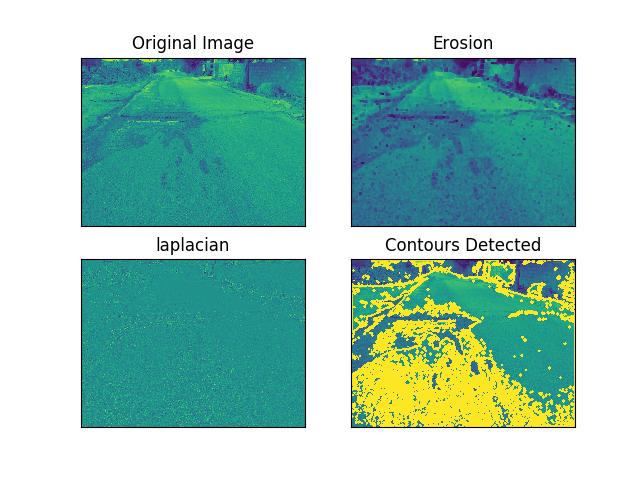
\includegraphics[width = 5in]{morph_transform_1}
        \caption{Output of Contour Detection using Morphological Transformation}
    \end{figure}
    \pagebreak
    
    \begin{figure}[ht!]
        \centering
        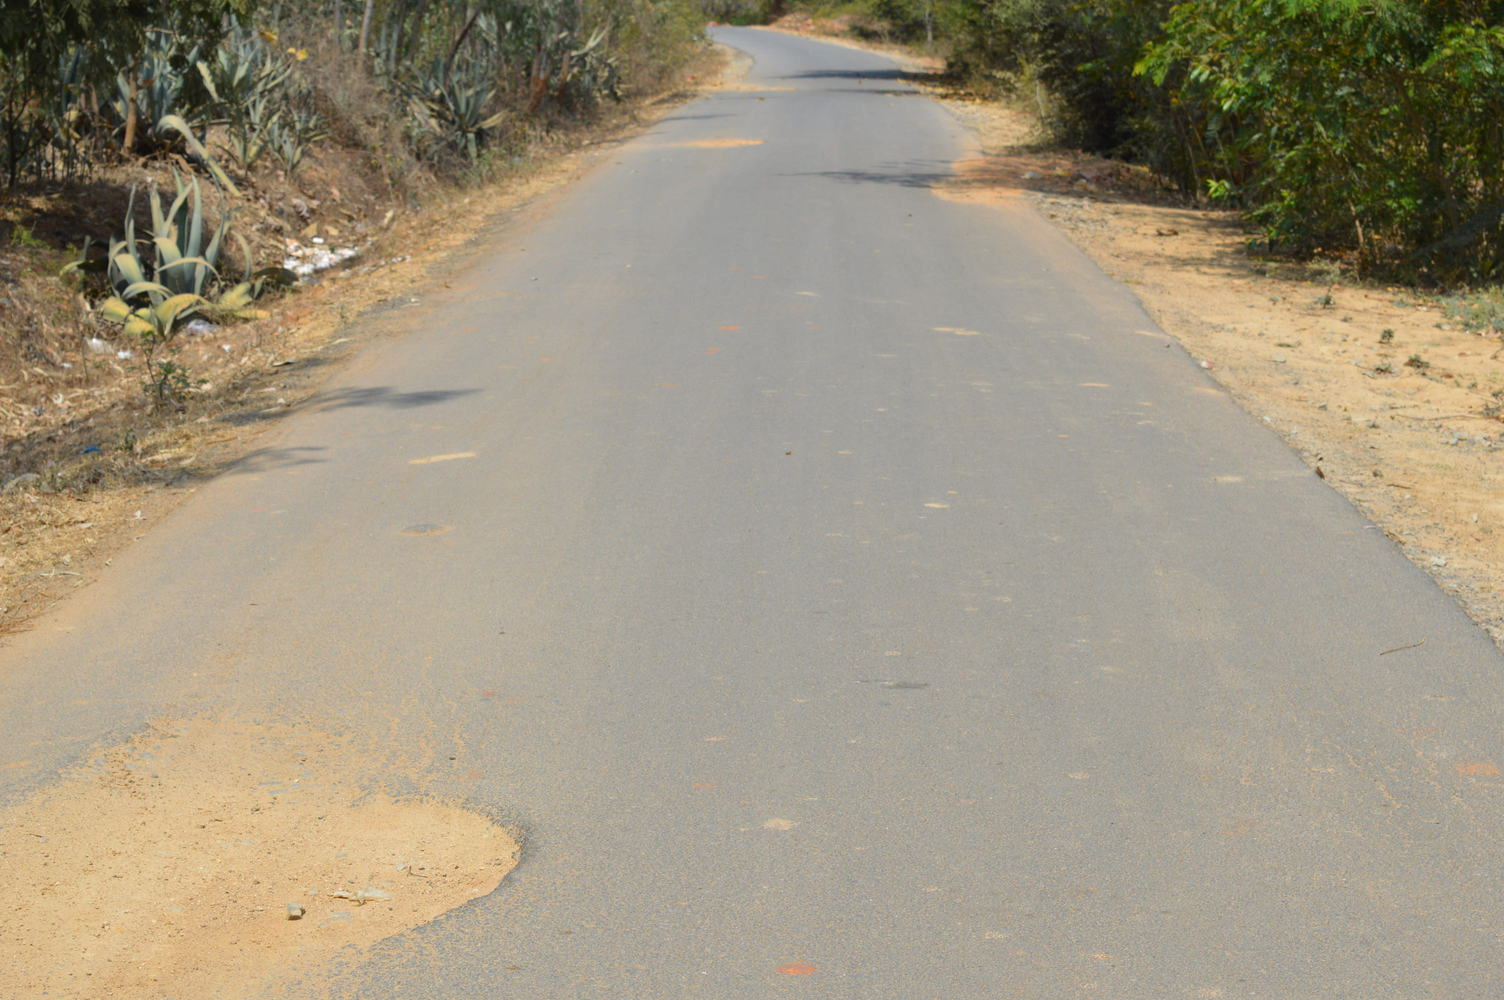
\includegraphics[width = 3in]{road_cam_31}
        \caption{Original Image from the Collected Dataset}
    \end{figure}

    \begin{figure}[ht!]
        \centering
        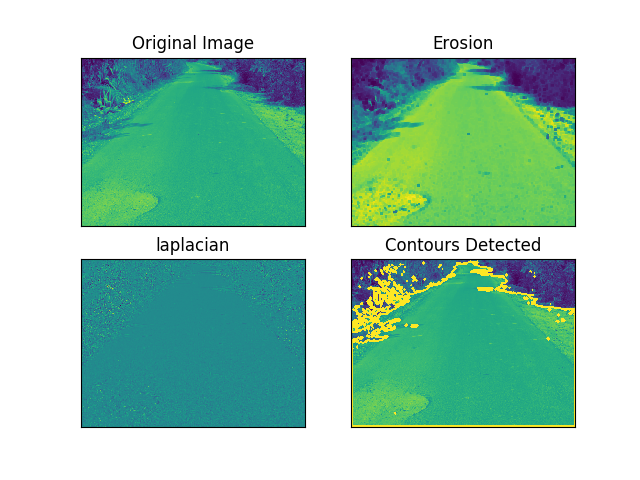
\includegraphics[width = 5in]{morph_transform_7}
        \caption{Output of Contour Detection using Morphological Transformation}
    \end{figure}
    \pagebreak
    
    \item \textbf{Method 5: Classic Watershed Algorithm}
    \begin{enumerate}
        \item In this methodolgy, we used the classic Watershed Algorithm for the segmentation. The Watershed Algorithm works as follows: The input image, being converted into the grayscale, is thresholded with Binary Inverse and Otsu's thresholding.The morphology transformations, opening and dilating, are applied to extract the background area from the image. To find the foreground area in the image, Distance Transform is being applied with L2 Transform as argument. Both the background and the foreground regions are marked and this output is fed to the \textbf{watershed} function to get the output of segmentation. This algorithm worked absolutely fine on the Google Images Dataset. It detected almost 90$\%$ of the potholes in our dataset along with the minor noise and the shadows.
    \end{enumerate}
    \begin{figure}[ht!]
        \centering
        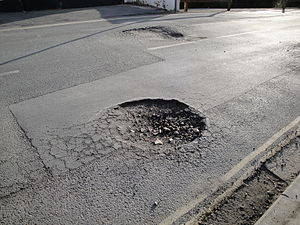
\includegraphics[width = 3in]{road_1}
        \caption{Original Image from the Collected Dataset}
    \end{figure}

    \begin{figure}[ht!]
        \centering
        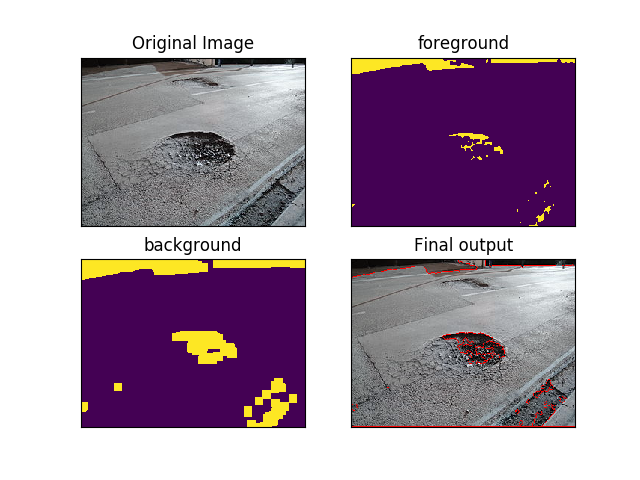
\includegraphics[width = 5in]{watershed_1}
        \caption{Output of Watershed Algorithm}
    \end{figure}
    \pagebreak
    
    \begin{figure}[ht!]
        \centering
        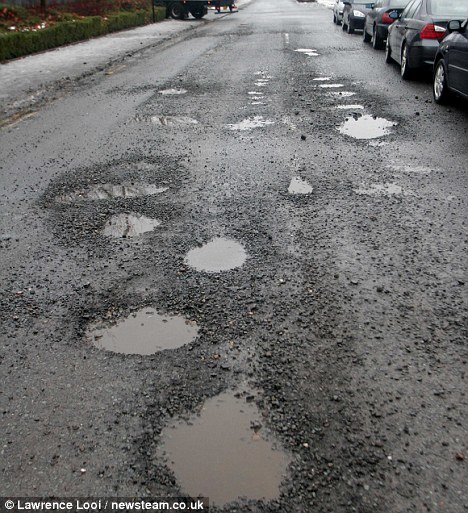
\includegraphics[width = 2in]{road_5}
        \caption{Original Image from the Collected Dataset}
    \end{figure}

    \begin{figure}[ht!]
        \centering
        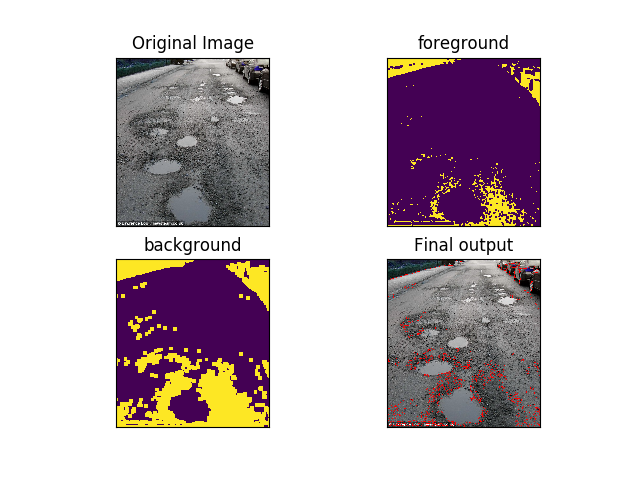
\includegraphics[width = 5in]{watershed_2}
        \caption{Output of Watershed Algorithm}
    \end{figure}
    \pagebreak
    
    \begin{figure}[ht!]
        \centering
        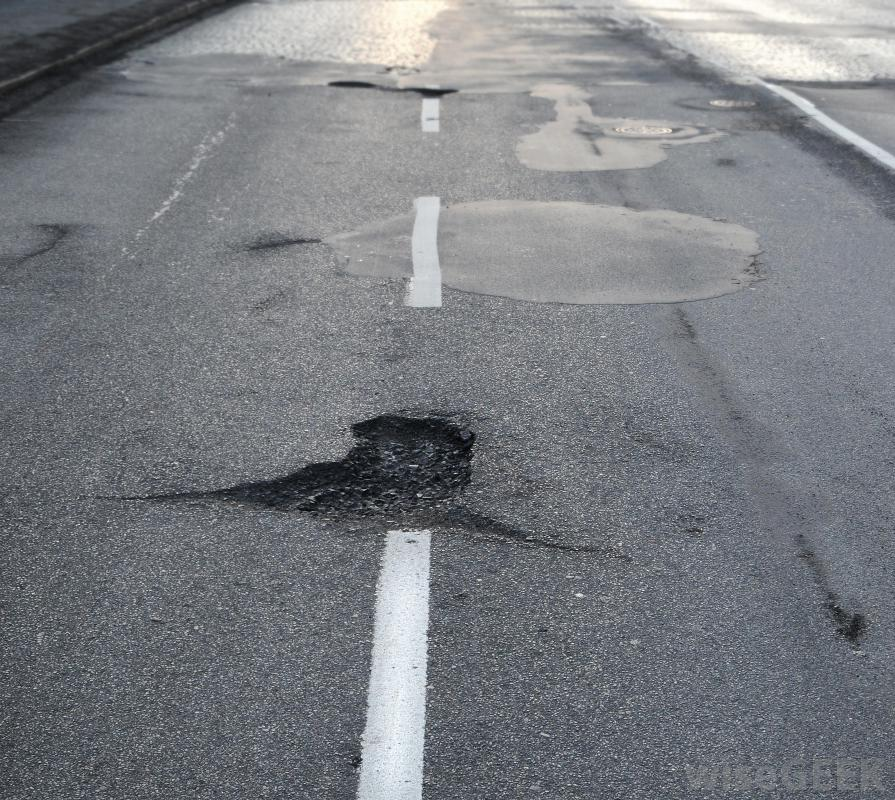
\includegraphics[width = 2in]{road_9}
        \caption{Original Image from the Collected Dataset}
    \end{figure}

    \begin{figure}[ht!]
        \centering
        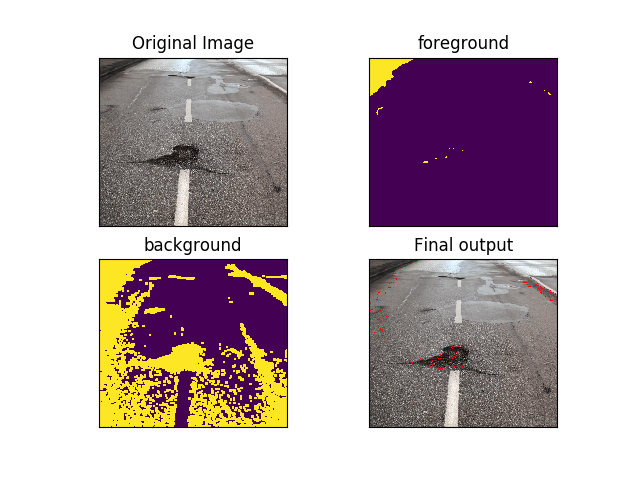
\includegraphics[width = 5in]{watershed_7}
        \caption{Output of Watershed Algorithm}
    \end{figure}
    \pagebreak
    
    \begin{figure}[ht!]
        \centering
        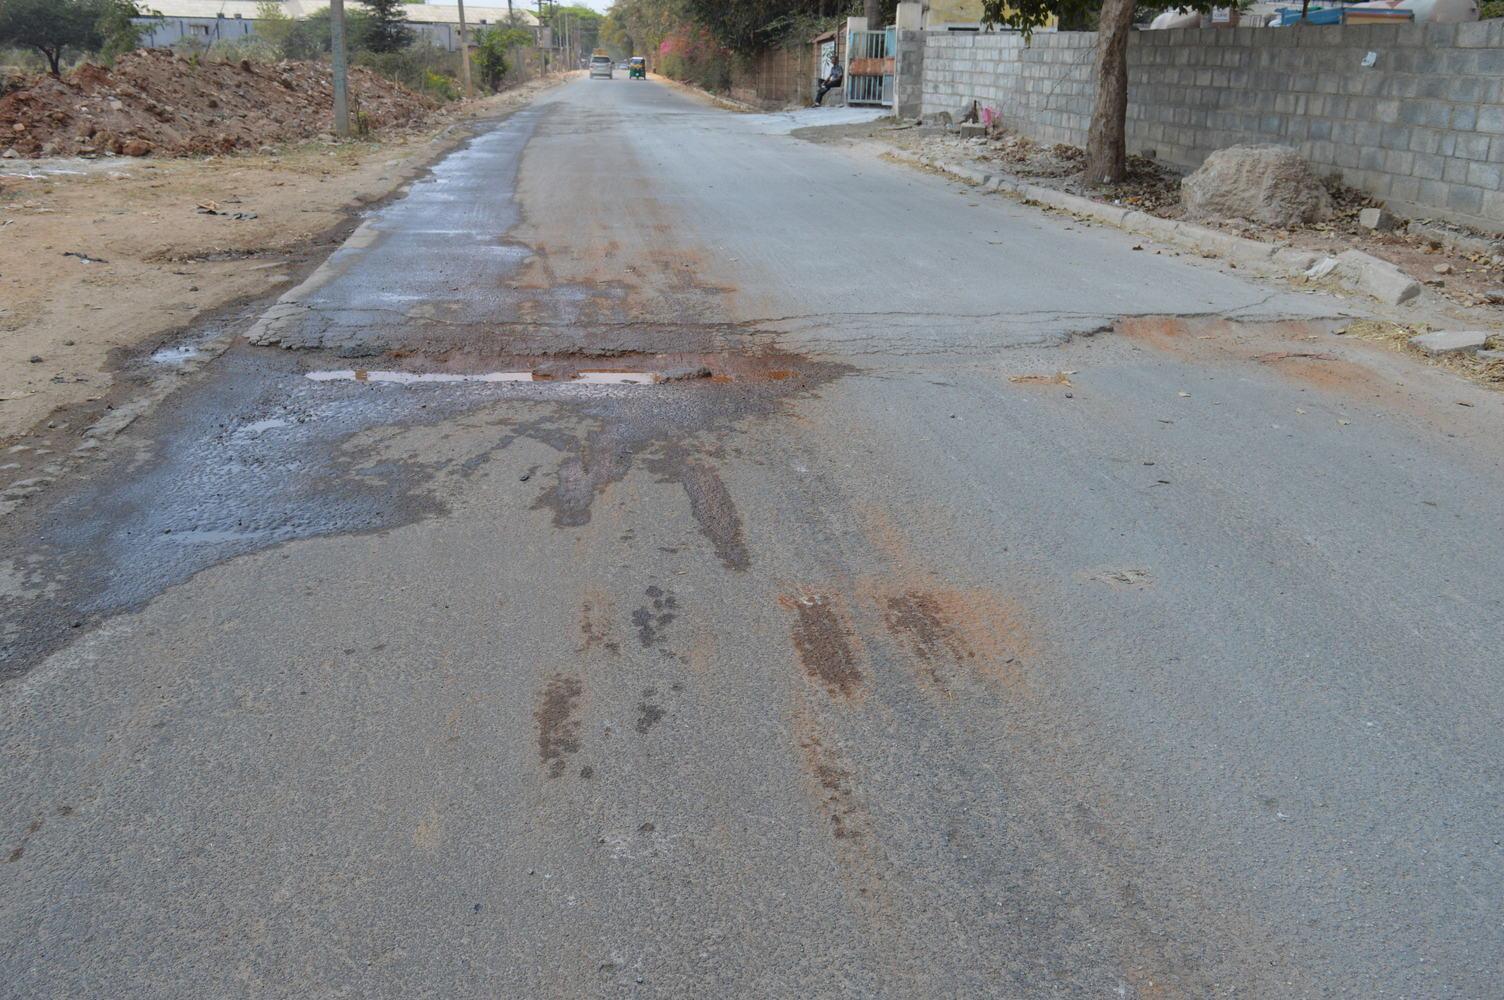
\includegraphics[width = 3in]{road_cam_4}
        \caption{Original Image from the Collected Dataset}
    \end{figure}

    \begin{figure}[ht!]
        \centering
        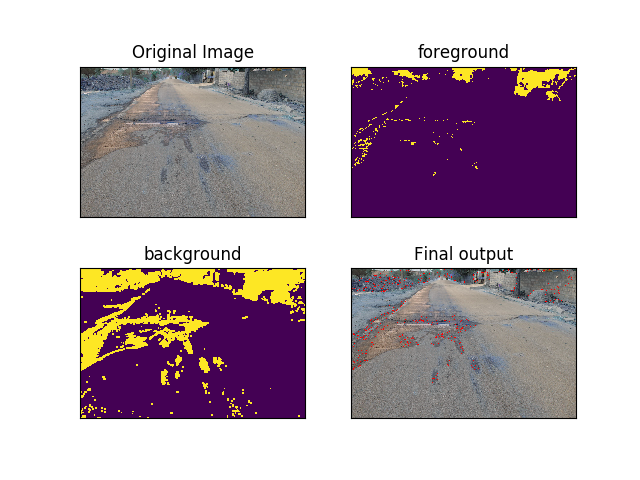
\includegraphics[width = 5in]{watershed_4}
        \caption{Output of Watershed Algorithm}
    \end{figure}
    \pagebreak
    
    \begin{figure}[ht!]
        \centering
        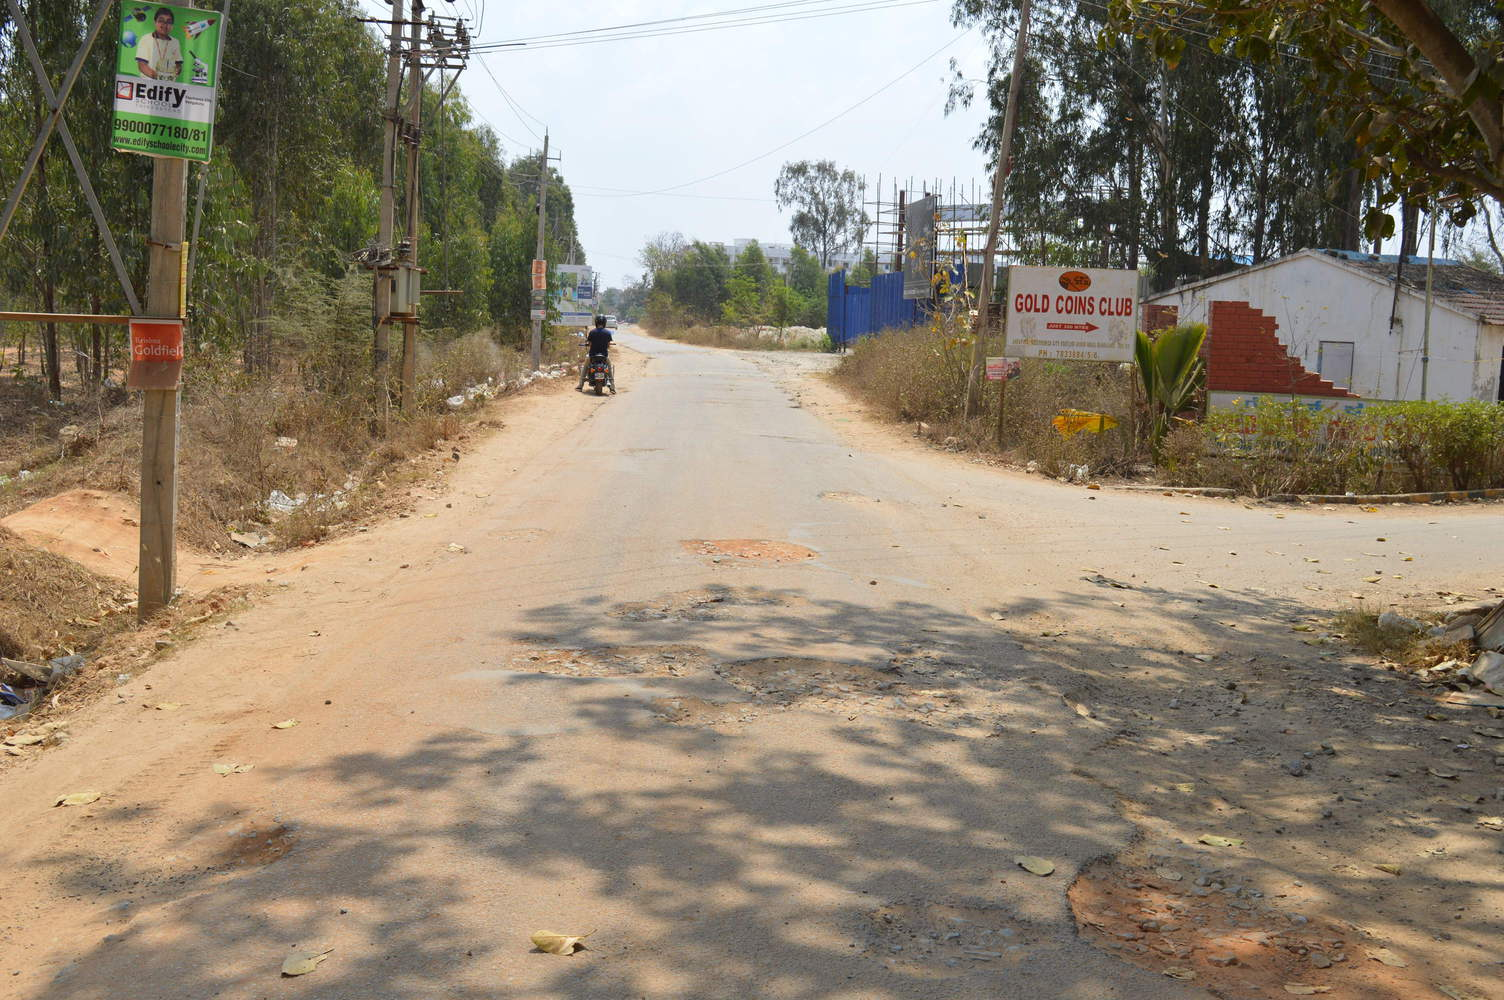
\includegraphics[width = 3in]{road_cam_20}
        \caption{Original Image from the Collected Dataset}
    \end{figure}

    \begin{figure}[ht!]
        \centering
        \includegraphics[width = 5in]{watershed_5}
        \caption{Output of Watershed Algorithm}
    \end{figure}
    \pagebreak
    
    \begin{figure}[ht!]
        \centering
        \includegraphics[width = 3in]{DSC_2529}
        \caption{Original Image from the Collected Dataset}
    \end{figure}

    \begin{figure}[ht!]
        \centering
        \includegraphics[width = 5in]{watershed_6}
        \caption{Output of Watershed Algorithm}
    \end{figure}
    \pagebreak
    
    \begin{figure}[ht!]
        \centering
        \includegraphics[width = 3in]{DSC_2522}
        \caption{Original Image from the Collected Dataset}
    \end{figure}

    \begin{figure}[ht!]
        \centering
        \includegraphics[width = 5in]{watershed_3}
        \caption{Output of Watershed Algorithm}
    \end{figure}
    \pagebreak
    
    \item \textbf{Method 5: Potholes Detection using Nienabar's Paper}
    \begin{enumerate}
        \item This technique referred one of the papers we followed, by the author Nienabar, Boysoon and Kroon. The input frame was to be converted to one of the color channels for the next steps. The results of Grayscale, Hue, saturation and variance channels were compared. Among these, the results came out best with the saturation channel. Gaussian Filter and Canny Edge Detection were applied to detect the edges. Finally, dilation was performed on the output frames, in 4 iterations, to bring out the edges/contours around potholes.
        Among all the methodologies being used, this methodology gave the best results both on the Google Images dataset and our dataset, despite of the shadow and illumination setbacks.
    \end{enumerate}
    \begin{figure}[ht!]
        \centering
        \includegraphics[width = 2in]{road_5}
        \caption{Original Image from the Google Images Dataset}
    \end{figure}

    \begin{figure}[ht!]
        \centering
        \includegraphics[width = 5in]{nienabar_2}
        \caption{Output of Nienabar's Algorithm}
    \end{figure}
    \pagebreak
    
    \begin{figure}[ht!]
        \centering
        \includegraphics[width = 2in]{road_8}
        \caption{Original Image from the Google Images Dataset}
    \end{figure}

    \begin{figure}[ht!]
        \centering
        \includegraphics[width = 5in]{nienabar_3}
        \caption{Output of Nienabar's Algorithm}
    \end{figure}
    \pagebreak
    
    \begin{figure}[ht!]
        \centering
        \includegraphics[width = 3in]{road_cam_34}
        \caption{Original Image from the Collected Images Dataset}
    \end{figure}

    \begin{figure}[ht!]
        \centering
        \includegraphics[width = 5in]{nienabar_1}
        \caption{Output of Nienabar's Algorithm}
    \end{figure}
    \pagebreak
    
    \begin{figure}[ht!]
        \centering
        \includegraphics[width = 3in]{road_cam_23}
        \caption{Original Image from the Collected Images Dataset}
    \end{figure}

    \begin{figure}[ht!]
        \centering
        \includegraphics[width = 5in]{nienabar_4}
        \caption{Output of Nienabar's Algorithm}
    \end{figure}
    \pagebreak
    
    \begin{figure}[ht!]
        \centering
        \includegraphics[width = 3in]{road_cam_4}
        \caption{Original Image from the Collected Images Dataset}
    \end{figure}

    \begin{figure}[ht!]
        \centering
        \includegraphics[width = 5in]{nienabar_5}
        \caption{Output of Nienabar's Algorithm}
    \end{figure}
    \pagebreak
    
    \begin{figure}[ht!]
        \centering
        \includegraphics[width = 3in]{road_cam_8}
        \caption{Original Image from the Collected Images Dataset}
    \end{figure}

    \begin{figure}[ht!]
        \centering
        \includegraphics[width = 5in]{nienabar_6}
        \caption{Output of Nienabar's Algorithm}
    \end{figure}
    \pagebreak
    
    \begin{figure}[ht!]
        \centering
        \includegraphics[width = 3in]{road_cam_16}
        \caption{Original Image from the Collected Images Dataset}
    \end{figure}

    \begin{figure}[ht!]
        \centering
        \includegraphics[width = 5in]{nienabar_8}
        \caption{Output of Nienabar's Algorithm}
    \end{figure}
    \pagebreak
\end{enumerate}
\end{document}
